\clearpage
\setcounter{table}{0}
\setcounter{figure}{0}
\renewcommand{\thetable}{S\arabic{table}}
\renewcommand{\thefigure}{S\arabic{figure}}
\section*{Supplementary Material}

This section collects additional hardware and software figures, supplementary NILM tables and figures (per-appliance results, layer and receptive-field derivations, post-processing, robustness and adaptation, operator fusion and the ARM build), the forecast outage analysis, the failure-mode and privacy-threat tables, and the detailed test designs, configurations and budgets that support the harmonic and forecasting results.
\subsection*{Additional hardware figures}

\begin{figure}[H]
    \centering
    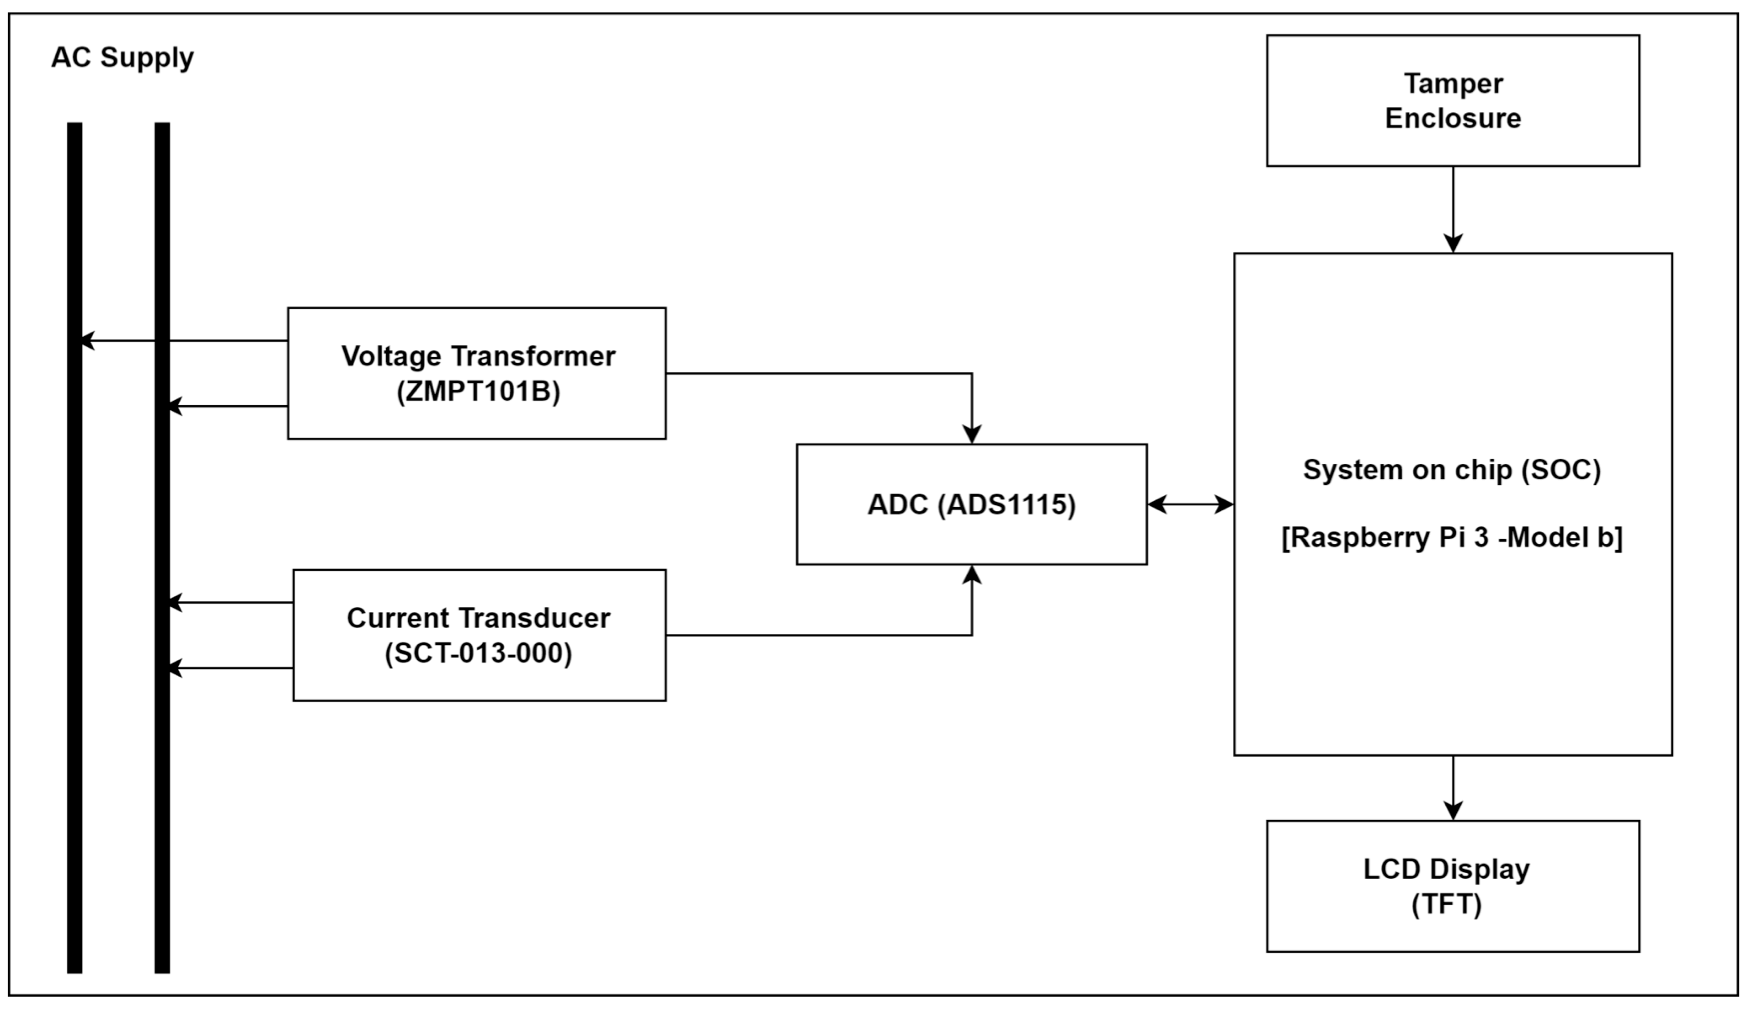
\includegraphics[width=0.90\textwidth]{figures/img3.png}
    \caption{First Generation NGSM Hardware Components illustrating the interface between the Raspberry Pi 3 and discrete analog sensors.}
    \label{fig:gen1_block}
\end{figure}

\begin{figure}[H]
    \centering
    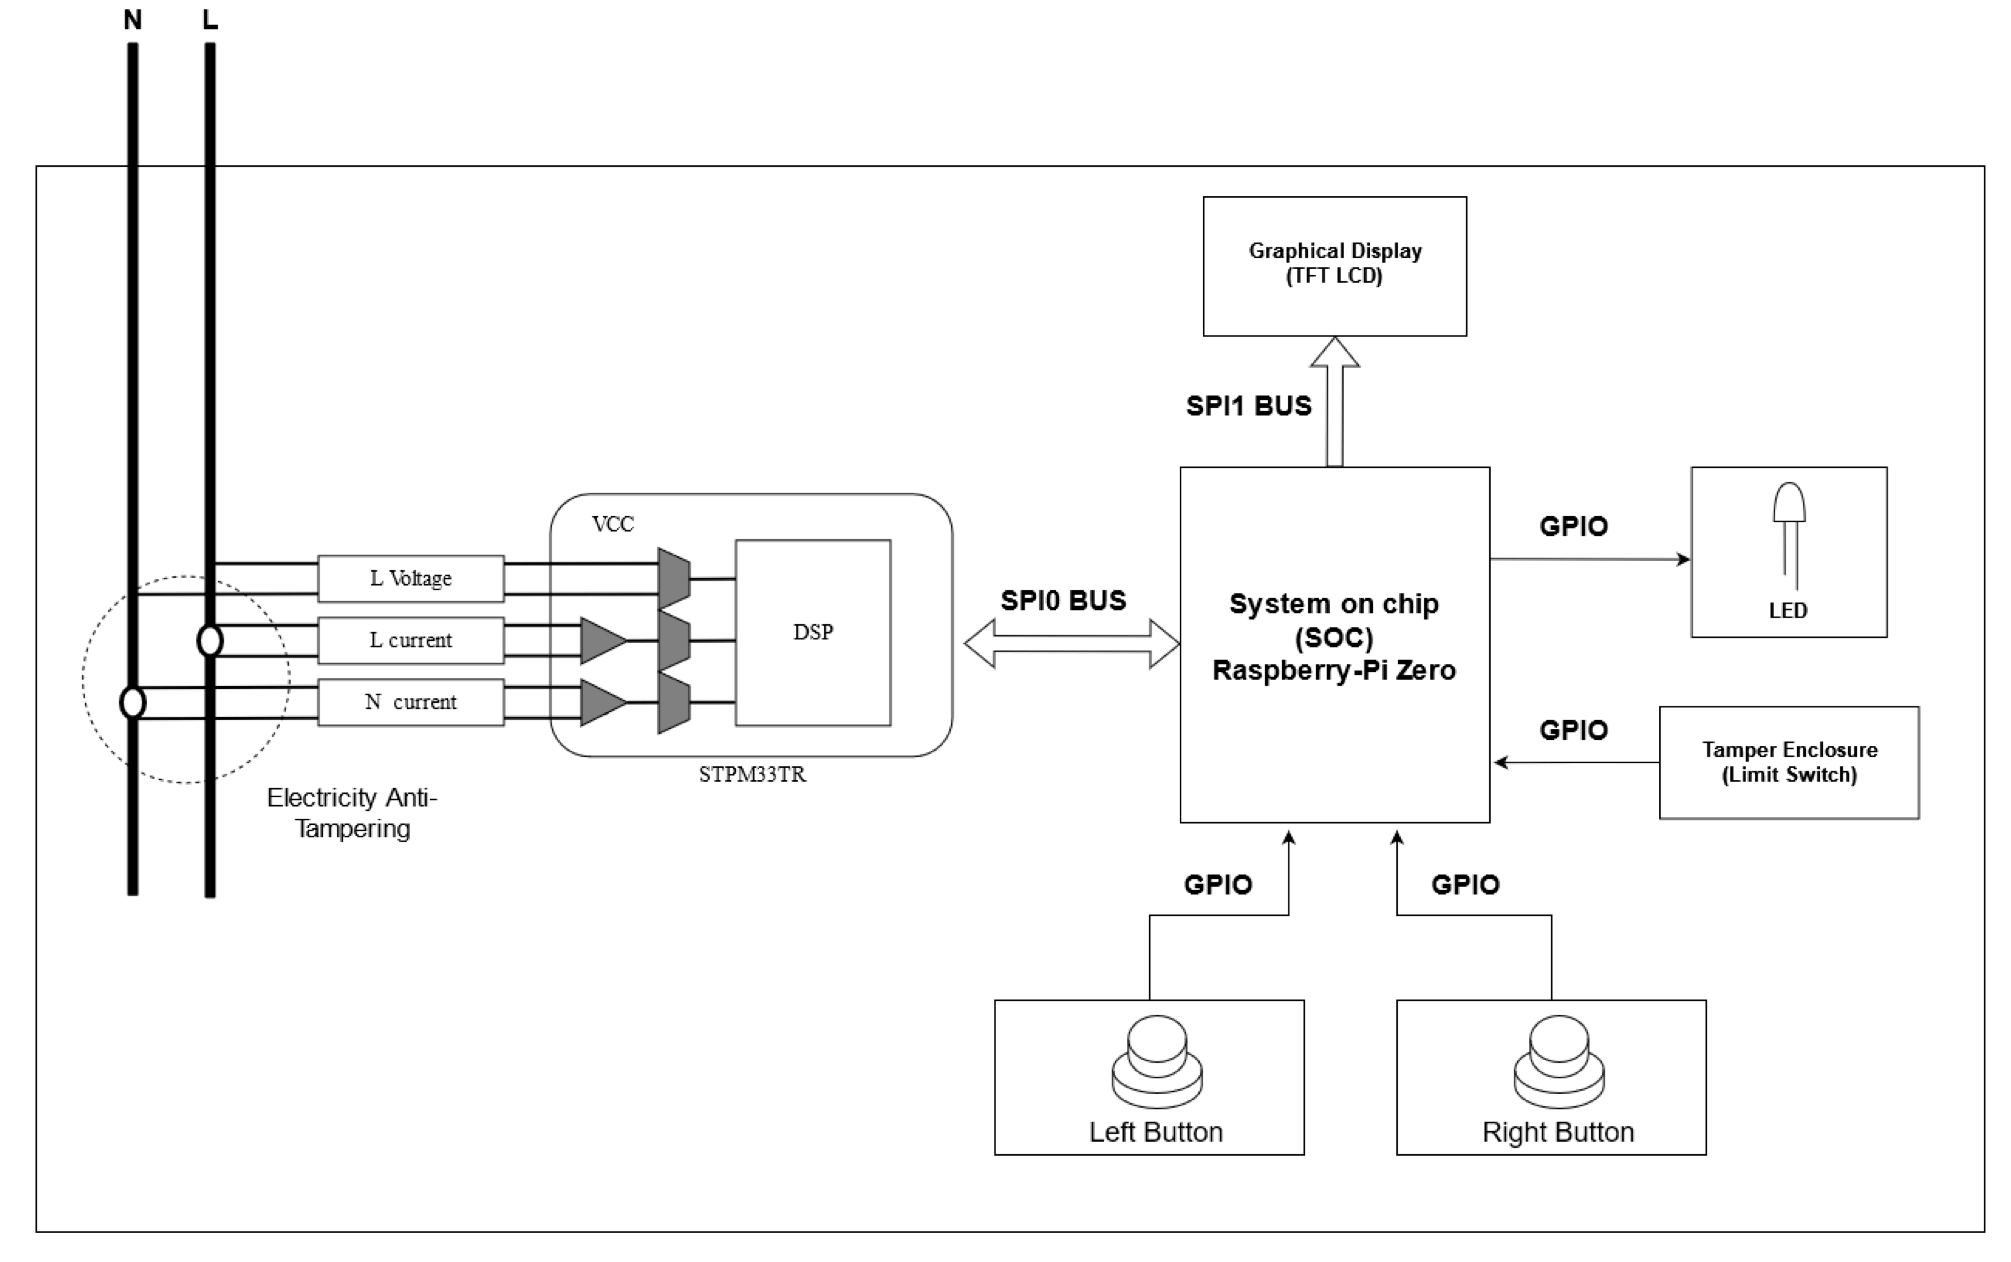
\includegraphics[width=0.90\textwidth]{figures/img7.png}
    \caption{Second Generation NGSM Hardware Components illustrating the integration of the Raspberry Pi Zero 2W with the STPM33 and TFT Display.}
    \label{fig:gen2_hardware}
\end{figure}

\begin{figure}[H]
    \centering
    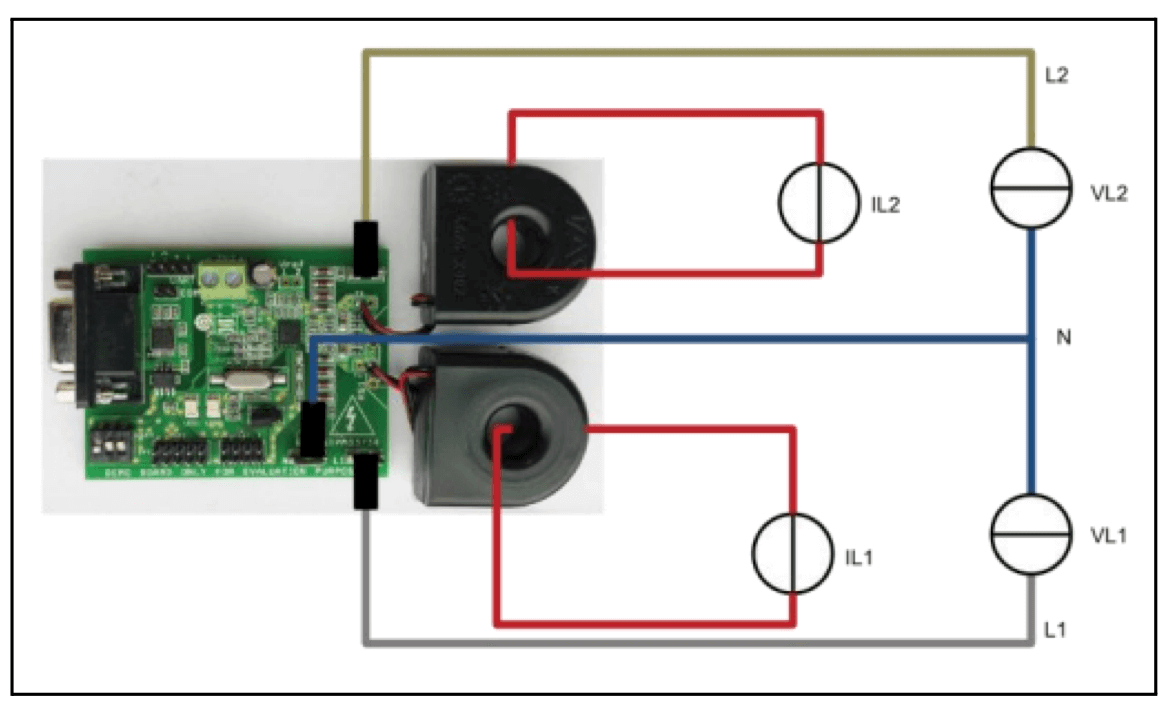
\includegraphics[width=0.50\textwidth]{figures/img8.png}
    \caption{Board connection diagram showing the dual-phase system interface and phantom load configuration.}
    \label{fig:gen2_connection}
\end{figure}

\begin{figure}[H]
    \centering
    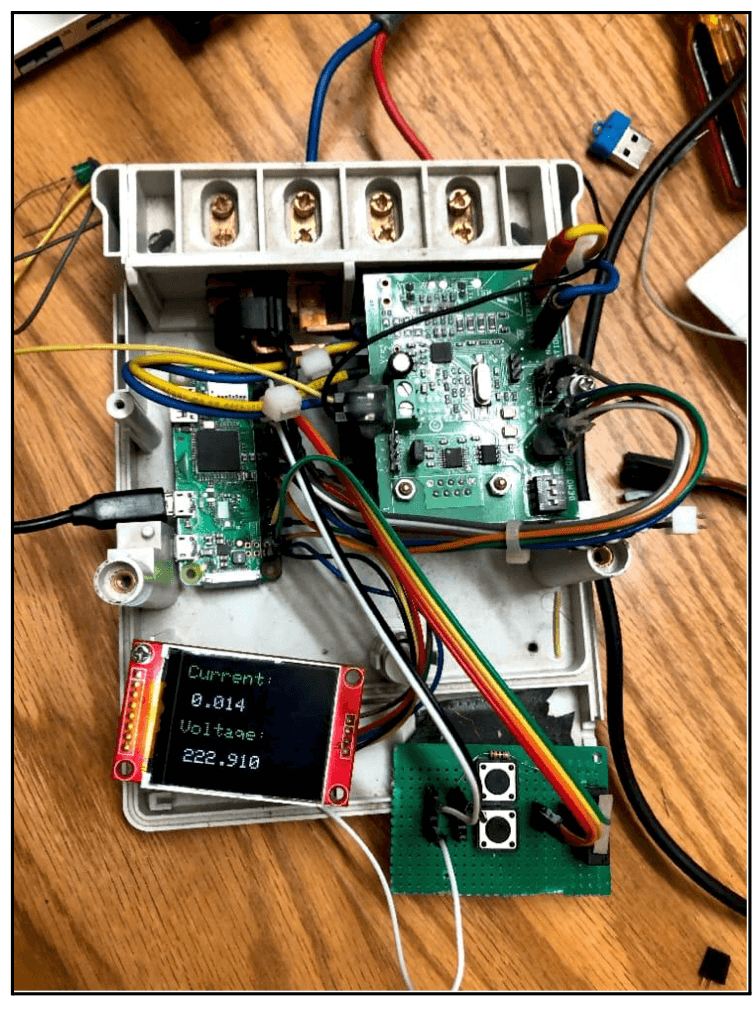
\includegraphics[width=0.48\textwidth]{figures/img9.png}
    \caption{TFT Display output: Measuring without input (Idle state).}
    \label{fig:gen2_idle}
\end{figure}

\begin{figure}[H]
    \centering
    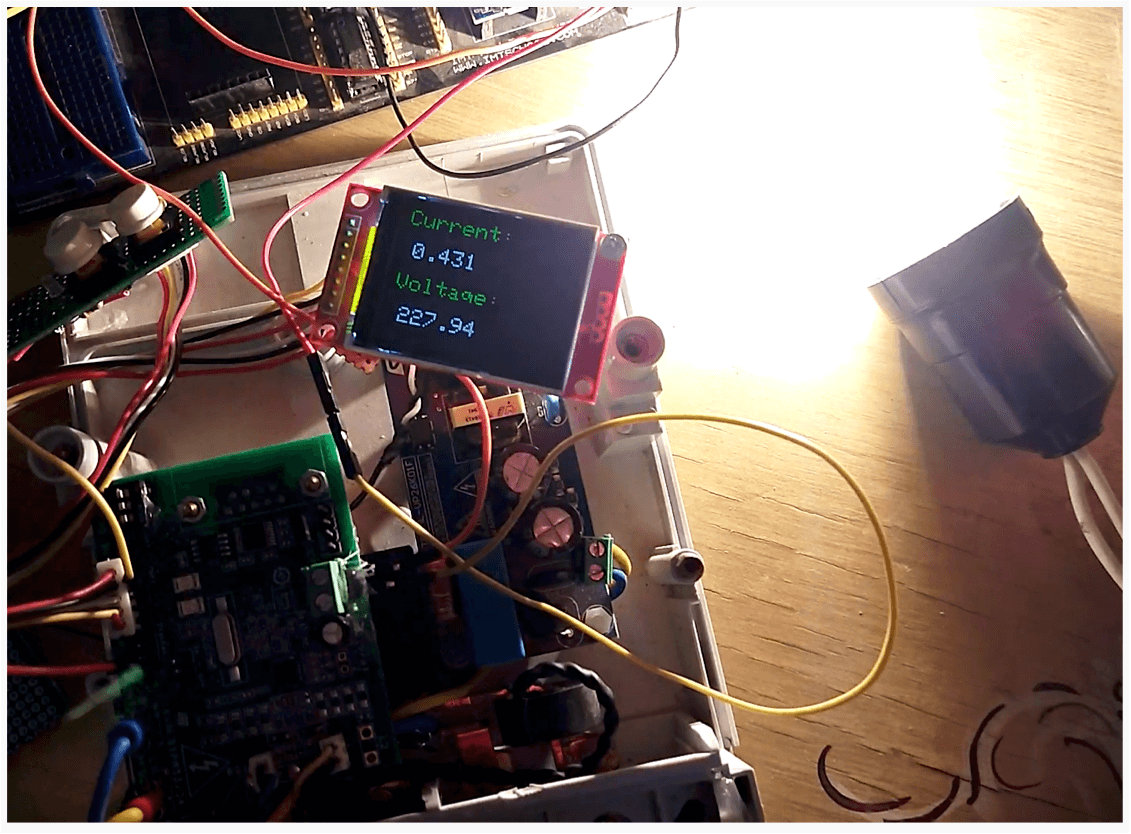
\includegraphics[width=0.50\textwidth]{figures/img10.png}
    \caption{TFT Display output: Measuring active load.}
    \label{fig:gen2_load}
\end{figure}

\begin{figure}[H]
    \centering
    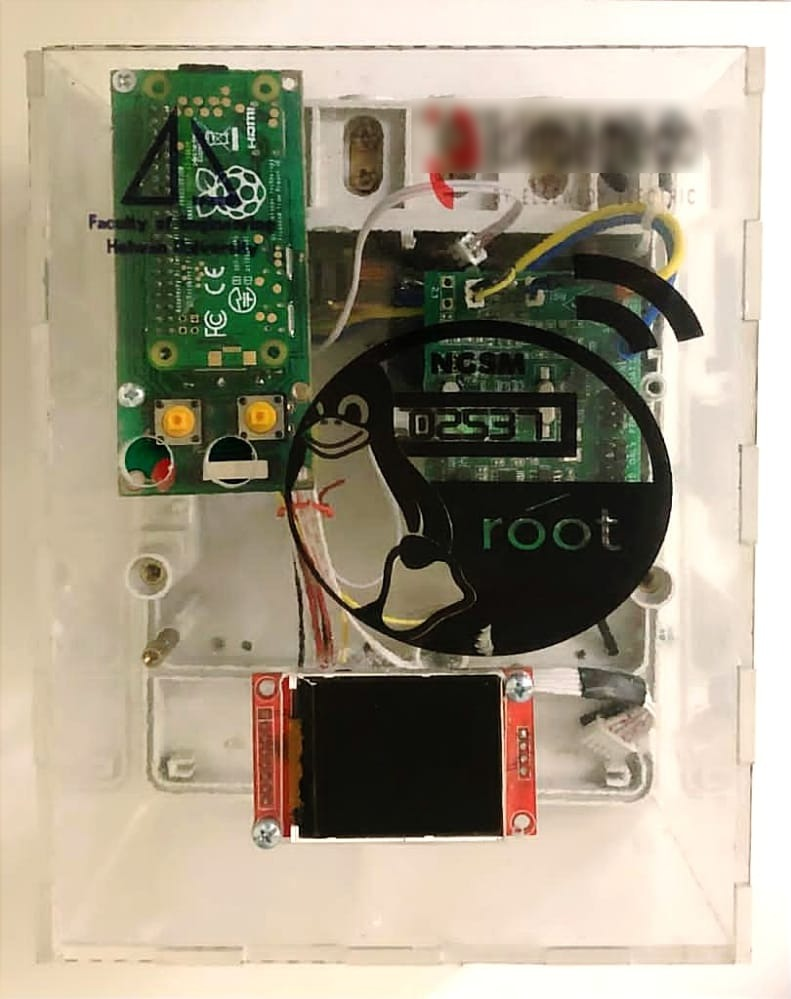
\includegraphics[width=0.48\textwidth]{figures/2ndgen.jpg}
    \caption{Final Second Generation hardware configuration showing the Raspberry Pi Zero 2W connected to the TFT display.}
    \label{fig:gen2_final}
\end{figure}


\begin{figure}[H]
    \centering
    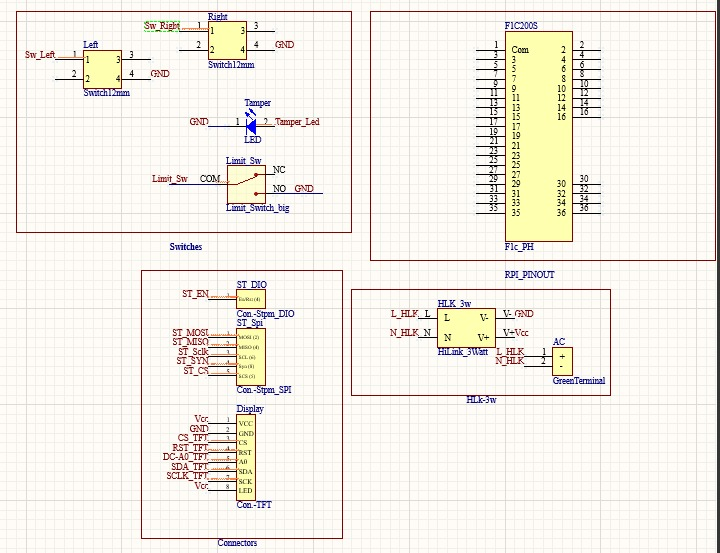
\includegraphics[width=0.85\textwidth]{figures/gen3_pcb_schematic.jpg}
    \caption{Schematic of the third-generation carrier PCB: F1C200s (MangoPi) connections, STPM33 and TFT connectors, switches and indicator LED, and the Hi-Link AC/DC converter.}
    \label{fig:gen3_pcb_schematic}
\end{figure}

\begin{figure}[H]
    \centering
    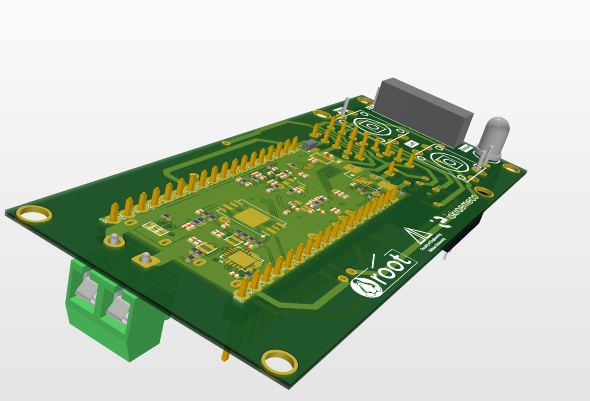
\includegraphics[width=0.60\textwidth]{figures/gen3_pcb_3d.png}
    \caption{3D model of the third-generation custom PCB with the MangoPi board soldered onto it.}
    \label{fig:gen3_pcb_3d}
\end{figure}

\subsection*{Software and user-interface figures}

\begin{figure}[H]
    \centering
    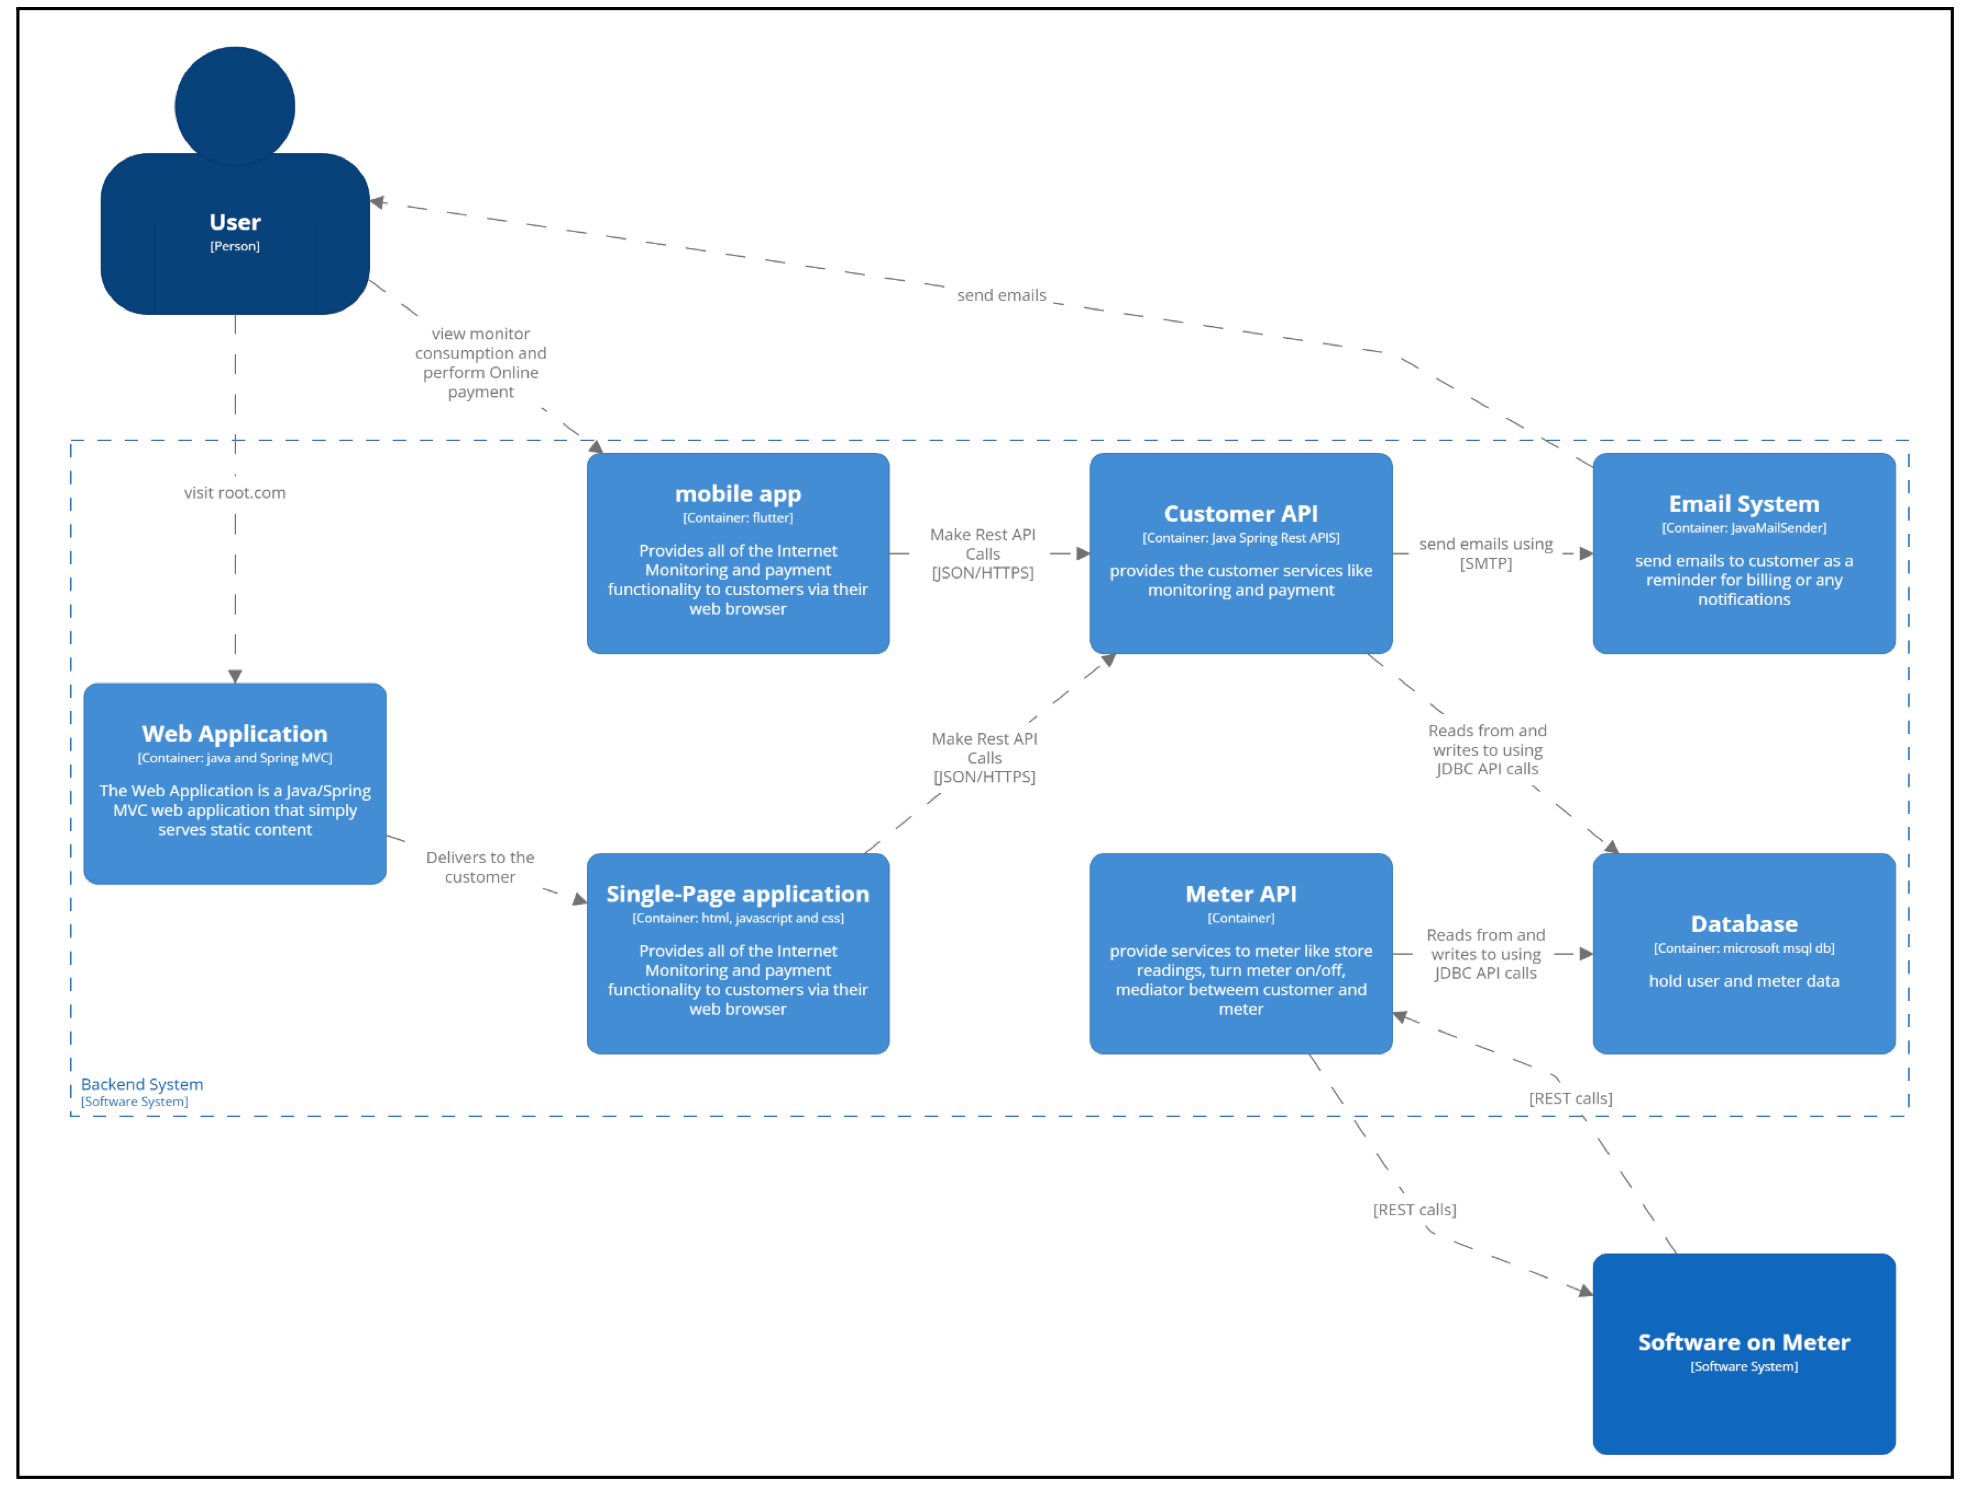
\includegraphics[width=0.90\textwidth]{figures/img13.png}
    \caption{Detailed NGSM Web-Based System Architecture showing the API interaction between the Meter Firmware, Cloud Backend, and Client Applications.}
    \label{fig:web_arch}
\end{figure}

\begin{figure}[H]
    \centering
    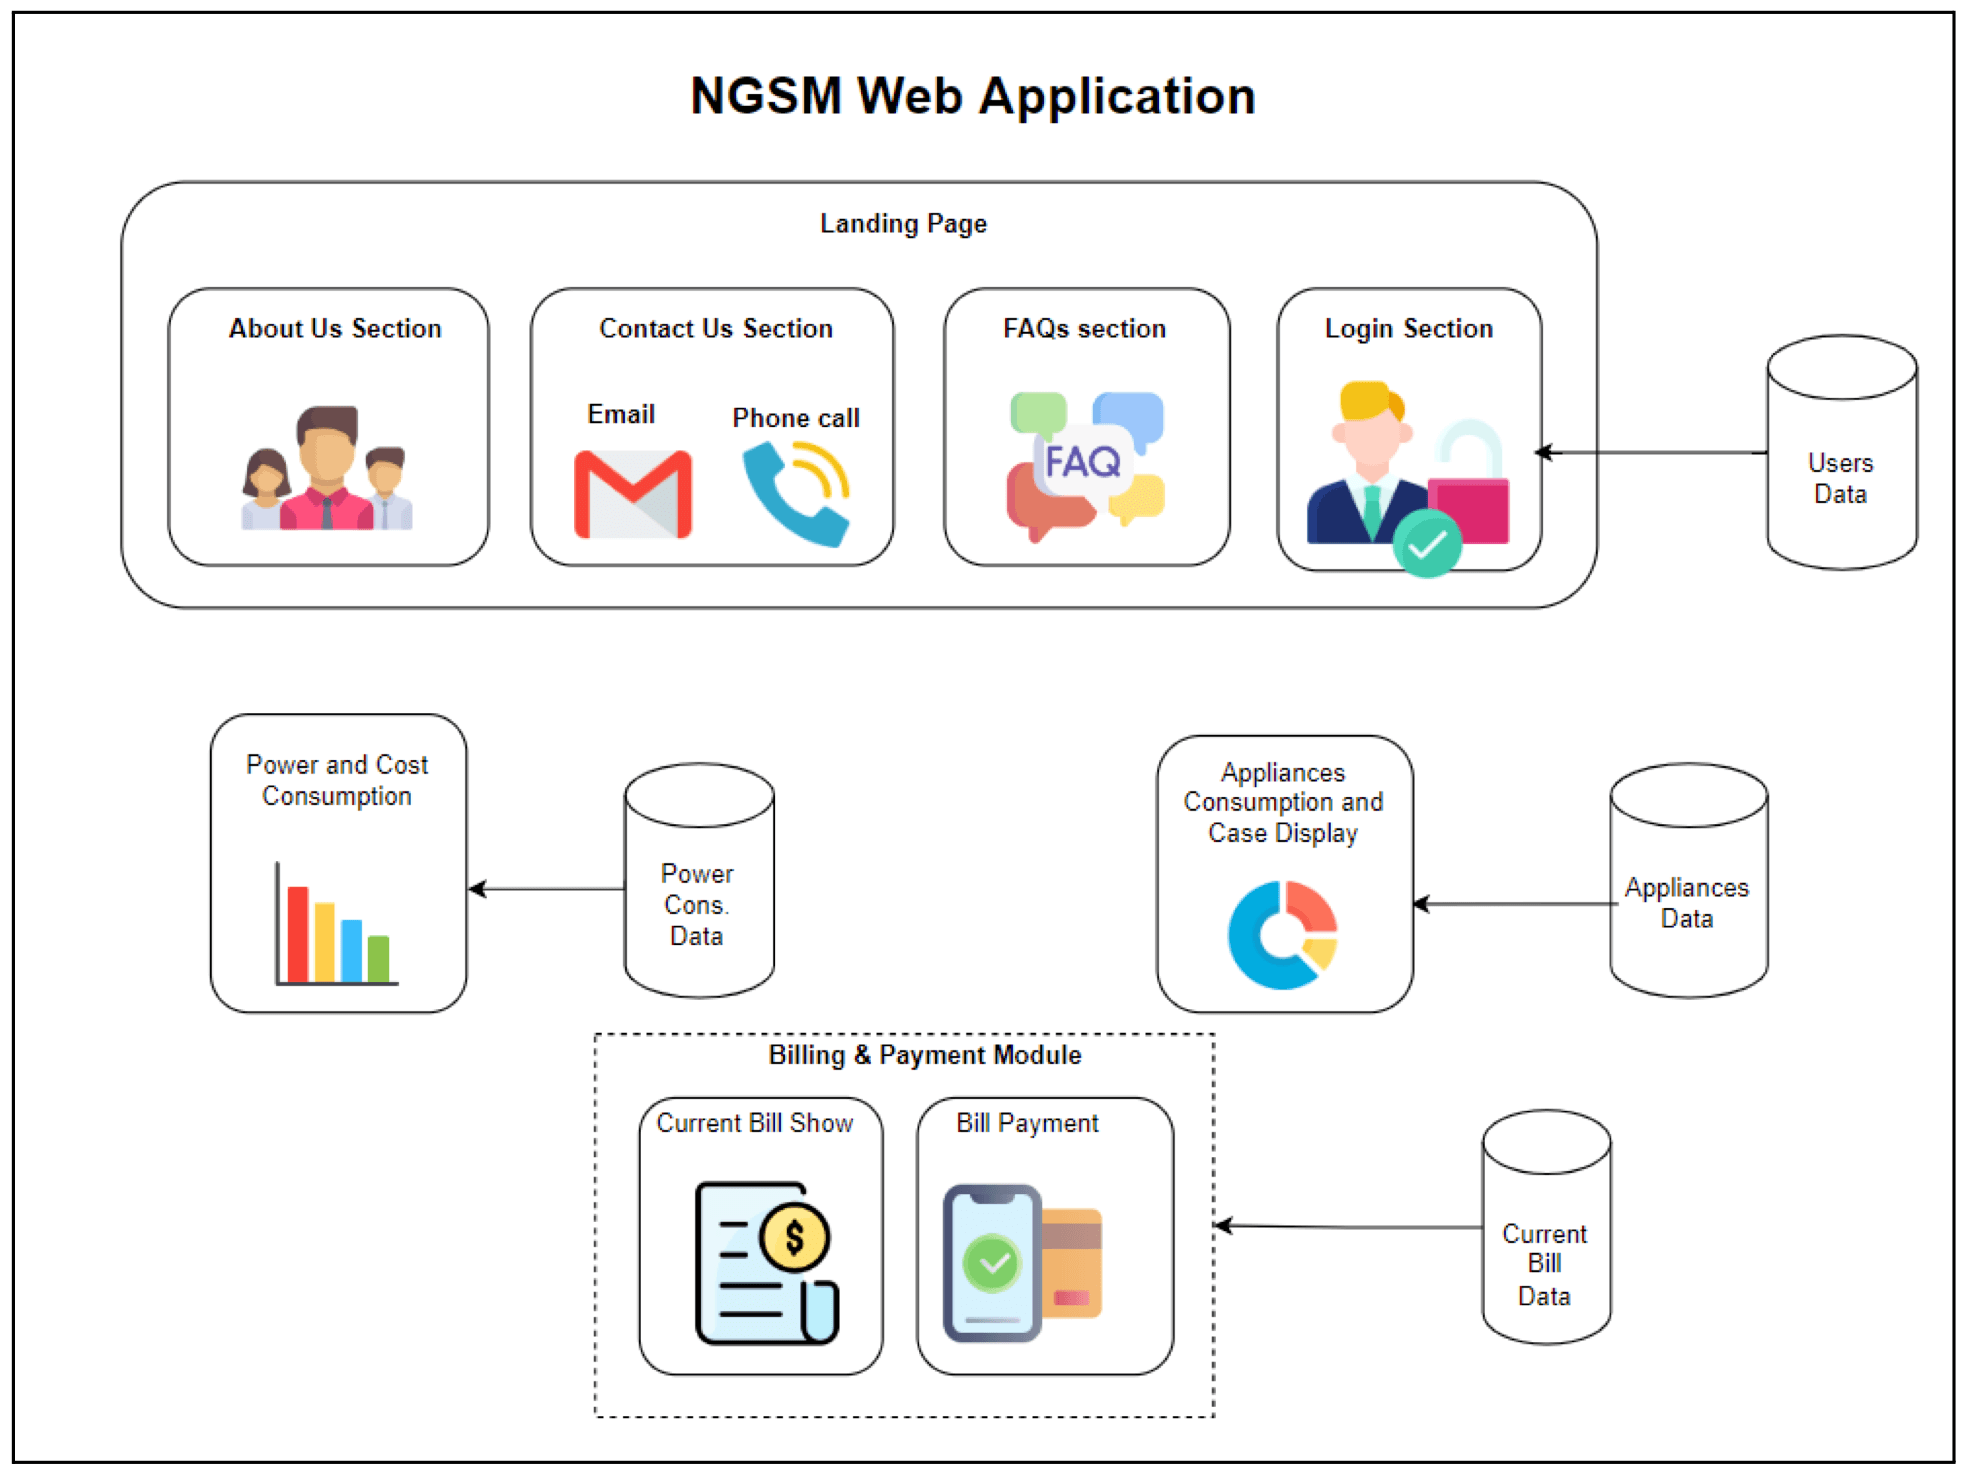
\includegraphics[width=0.85\textwidth]{figures/img14.png}
    \caption{User Interaction Flow Diagram illustrating the navigation paths between public pages, authentication layers, and private dashboard modules.}
    \label{fig:user_flow}
\end{figure}

\begin{figure}[H]
    \centering
    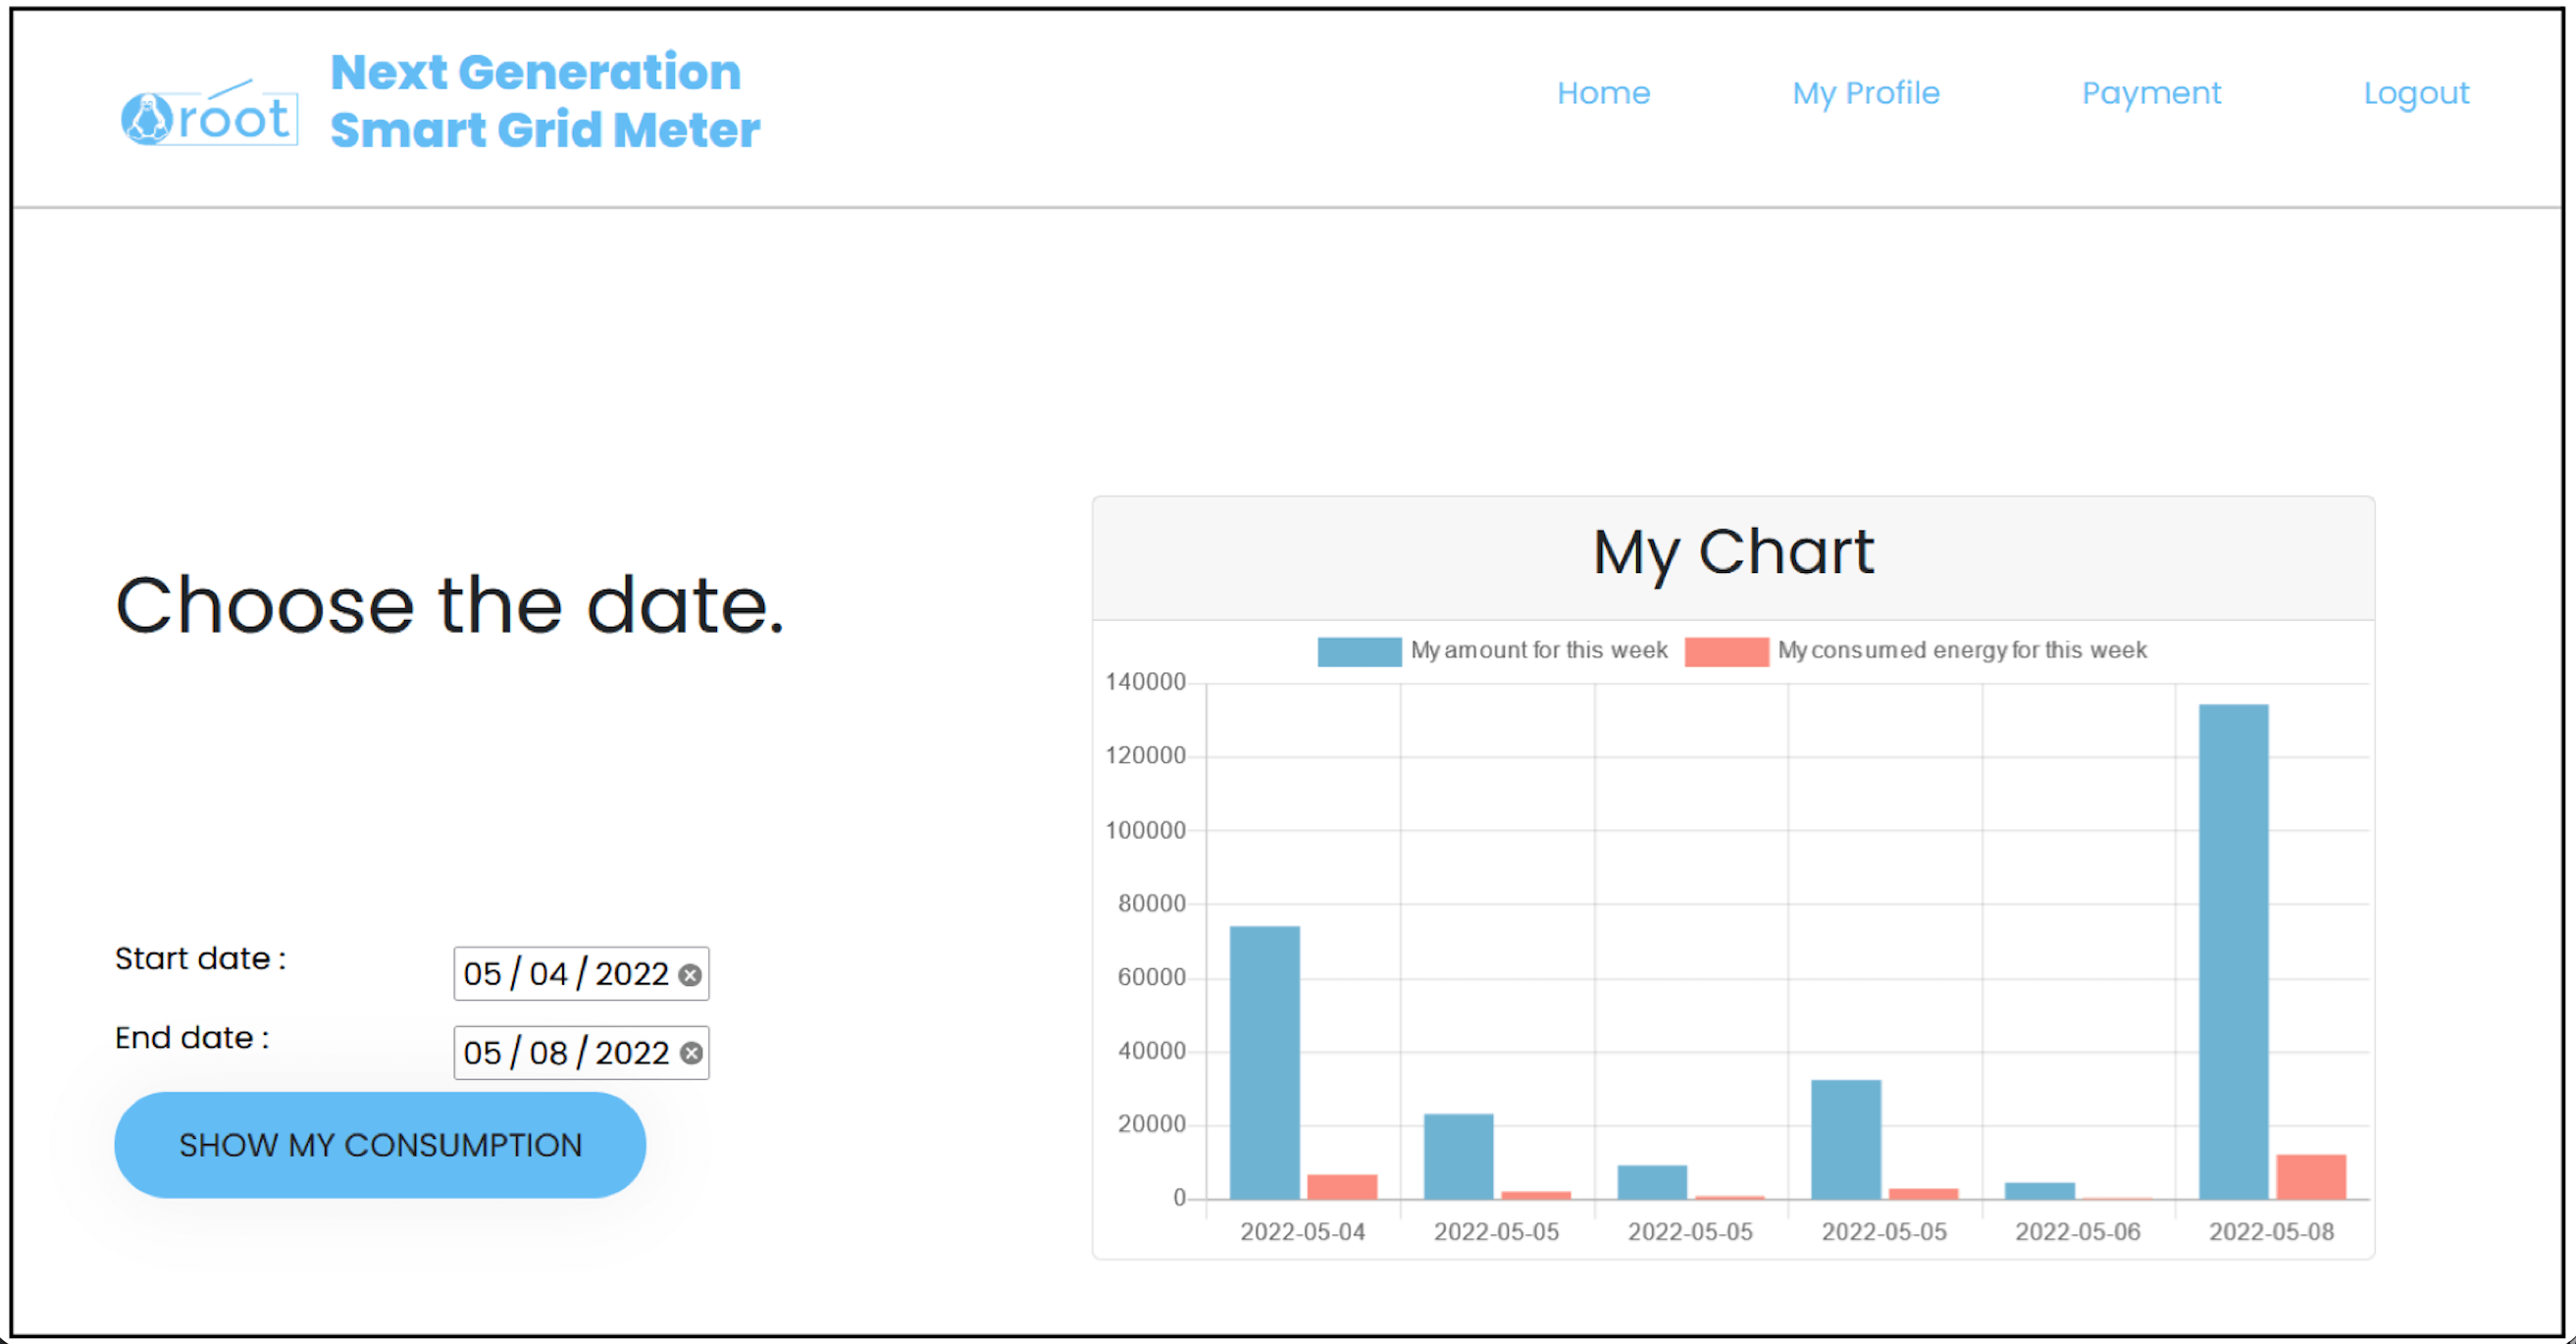
\includegraphics[width=0.85\textwidth]{figures/img16.png}
    \caption{Energy Consumption Dashboard providing visualization of historical usage and cost metrics.}
    \label{fig:consumption_page}
\end{figure}

\begin{figure}[H]
    \centering
    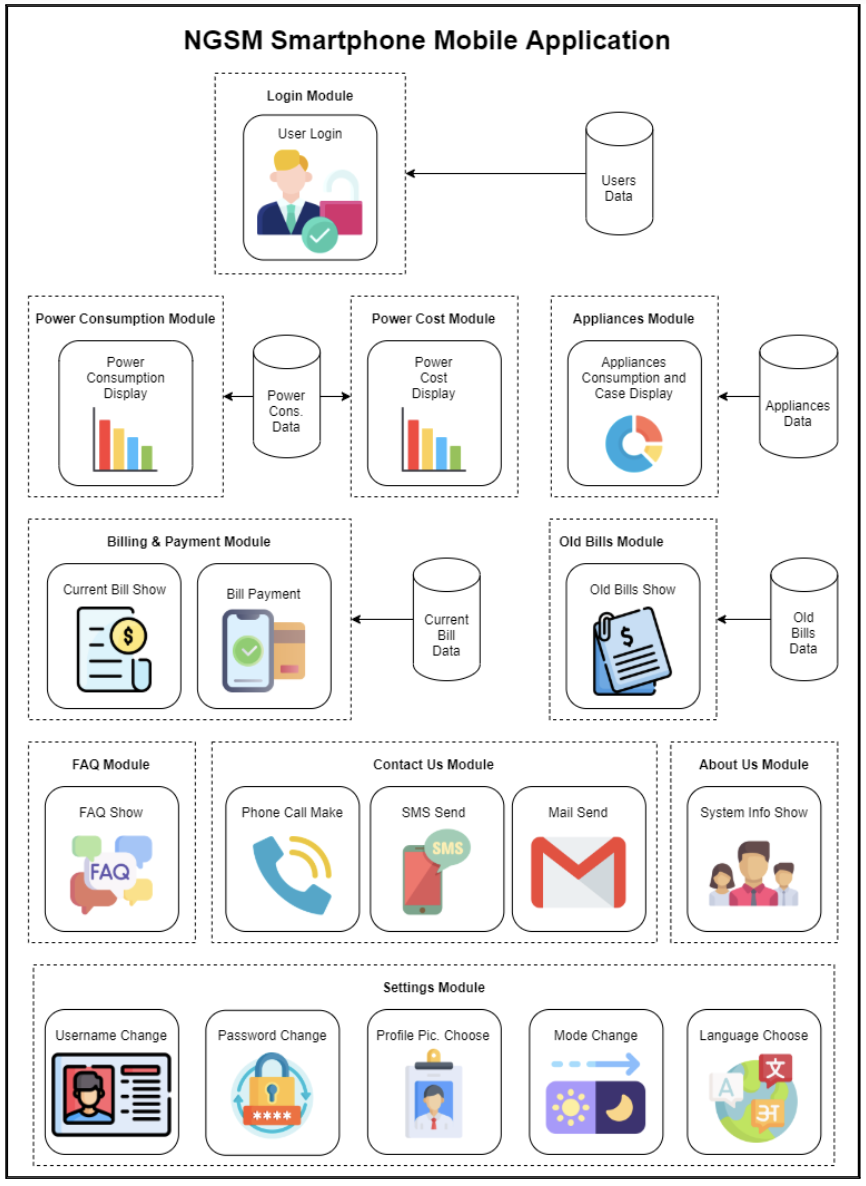
\includegraphics[width=0.50\textwidth]{figures/img18.png}
    \caption{Activity Diagram illustrating the operational flow of the NGSM Mobile Application.}
    \label{fig:mobile_activity}
\end{figure}

\begin{figure}[H]
    \centering
    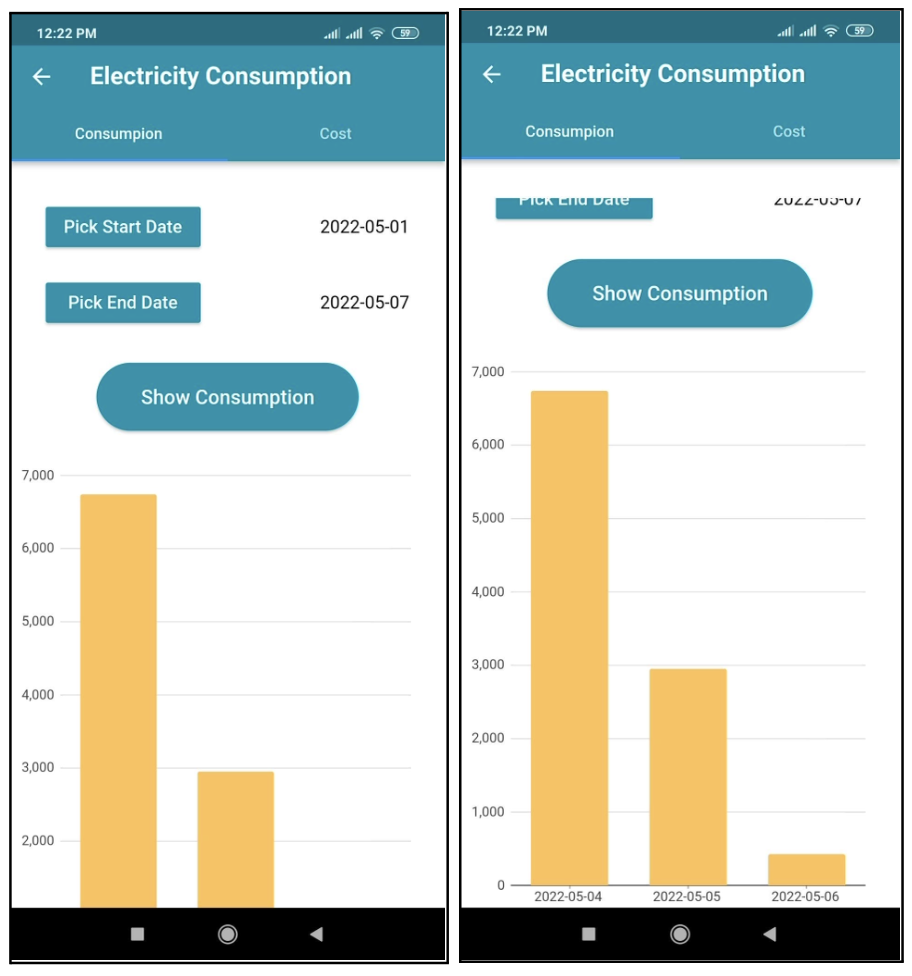
\includegraphics[width=0.50\textwidth]{figures/img21.png}
    \caption{Energy Consumption (kWh) View.}
    \label{fig:mobile_kwh}
\end{figure}

\begin{figure}[H]
    \centering
    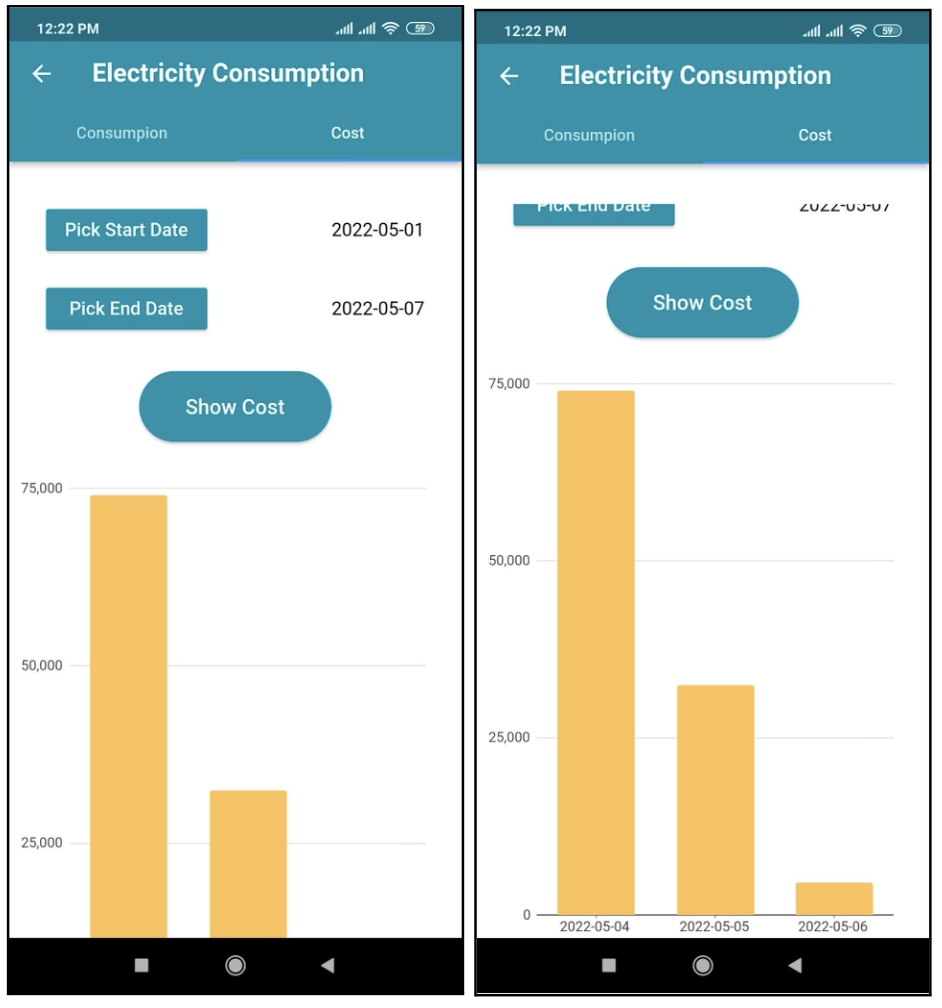
\includegraphics[width=0.50\textwidth]{figures/img22.png}
    \caption{Calculated Cost View.}
    \label{fig:mobile_cost}
\end{figure}


\subsection*{Additional NILM results}

\begin{table}[H]
\centering
\caption{Receptive-field derivation of the EDTCN ($K=3$, two convolutions per block, input projection of kernel 7). Time spans assume the 8~s sampling interval used for all datasets.}
\label{tab:rf}
\footnotesize
\begin{tabular}{@{}lcccc@{}}
\toprule
Stage & Dilation $d_i$ & Added steps & Cumulative $R$ & Span (min) \\
\midrule
Input projection (kernel 7) & 1 & 6 & 7 & 0.9 \\
TCN block 1 & 1 & 4 & 11 & 1.5 \\
TCN block 2 & 2 & 8 & 19 & 2.5 \\
TCN block 3 & 4 & 16 & 35 & 4.7 \\
TCN block 4 & 8 & 32 & 67 & 8.9 \\
TCN block 5 & 16 & 64 & 131 & 17.5 \\
TCN block 6 & 32 & 128 & \textbf{259} & \textbf{34.5} \\
\bottomrule
\end{tabular}
\end{table}

\begin{table}[H]
\centering
\caption{Layer-by-layer description of the EDTCN (REFIT configuration, 9 appliances, batch dimension omitted). MACs are counted per 512-step window; $A$ is the number of appliances.}
\label{tab:layers}
\footnotesize
\begin{adjustbox}{max width=\textwidth}\begin{tabular}{@{}llcccrr@{}}
\toprule
Block & Layers & Output size & Kernel & Dilation & Params & MACs (M) \\
\midrule
Input & aggregate power & $1\times512$ & -- & -- & -- & -- \\
Input projection & Conv1d$_{1\rightarrow128}$, BN, ReLU, Dropout(0.2) & $128\times512$ & 7 & 1 & 1,280 & 0.46 \\
TCN block 1 & 2$\times$[Conv1d$_{128\rightarrow128}$, BN] + ReLU, Dropout(0.2), residual add & $128\times512$ & 3 & 1 & 99,072 & 50.6 \\
TCN block 2 & same as block 1 & $128\times512$ & 3 & 2 & 99,072 & 50.9 \\
TCN block 3 & same as block 1 & $128\times512$ & 3 & 4 & 99,072 & 51.5 \\
TCN block 4 & same as block 1 & $128\times512$ & 3 & 8 & 99,072 & 52.7 \\
TCN block 5 & same as block 1 & $128\times512$ & 3 & 16 & 99,072 & 55.1 \\
TCN block 6 & same as block 1 & $128\times512$ & 3 & 32 & 99,072 & 59.8 \\
Output heads ($A$ in parallel) & Conv1d$_{128\rightarrow32}$, ReLU, Dropout(0.2), Conv1d$_{32\rightarrow1}$ & $A\times512$ & 3 / 1 & 1 & 12,353 per head & 6.3 per head \\
\midrule
Total ($A=9$) & & $512\times9$ & & & 706,889 & 377.8 \\
\bottomrule
\end{tabular}\end{adjustbox}
\end{table}

\begin{table}[H]
\centering
\caption{Per-appliance results of the deployed SustDataED2 model on the test split (304 windows). ON (\%) is the fraction of test time the appliance is above 15~W; SAE and NDE are undefined (--) for appliances that are never ON in the test split. Device types: A always-on/cycling, B regular-use, C burst. The precision, recall and F1 of the Fridge-Freezer and the Kettle agree to two decimals by coincidence (unrounded: 0.8818/0.9952/0.9350 and 0.8819/0.9957/0.9354); the Kettle is ON in only 0.7\% of the test time.}
\label{tab:SustDataED2_per_appliance}
\footnotesize
\begin{tabular}{@{}lcccccccc@{}}
\toprule
Appliance & Type & ON (\%) & MAE (W) & SAE (\%) & NDE & F1 & Prec. & Recall \\
\midrule
Fridge-Freezer & A & 24.9 & 6.68 & 9.5 & 0.08 & 0.935 & 0.882 & 0.995 \\
Freezer & A & 35.4 & 9.67 & 0.6 & 0.18 & 0.908 & 0.858 & 0.963 \\
TV-Philips & A & 0.0 & 5.41 & -- & -- & 0.000 & 0.000 & 0.000 \\
TV-Samsung & A & 5.2 & 9.77 & 84.3 & 0.80 & 0.000 & 0.000 & 0.000 \\
TV-Sharp & A & 0.0 & 6.49 & -- & -- & 0.000 & 0.000 & 0.000 \\
MacBookPro-1 & B & 0.0 & 1.82 & -- & -- & 0.000 & 0.000 & 0.000 \\
MacBookPro-2 & B & 0.0 & 1.20 & -- & -- & 0.000 & 0.000 & 0.000 \\
Kettle & C & 0.7 & 9.77 & 19.0 & 0.17 & 0.935 & 0.882 & 0.996 \\
Microwave & C & 7.2 & 7.93 & 20.3 & 0.08 & 0.434 & 0.790 & 0.300 \\
HairDryer-Straightener & C & 0.7 & 1.70 & 103.5 & 0.94 & 0.119 & 0.133 & 0.108 \\
CoffeeMachine & C & 0.1 & 1.02 & 55.6 & 0.97 & 0.059 & 0.033 & 0.275 \\
VacuumCleaner & C & 0.1 & 1.54 & 24.4 & 0.98 & 0.050 & 0.026 & 0.701 \\
\bottomrule
\end{tabular}
\end{table}

\begin{table}[H]
\centering
\caption{Per-appliance results of the deployed REFIT model on the unseen test houses 19--21 (59,927 windows). Device types follow the dataset package: A always-on/cycling, B regular-use, C burst.}
\label{tab:refit_per_appliance}
\footnotesize
\begin{tabular}{@{}lcccccccc@{}}
\toprule
Appliance & Type & ON (\%) & MAE (W) & SAE (\%) & NDE & F1 & Prec. & Recall \\
\midrule
Fridge & A & 37.1 & 34.15 & 46.8 & 0.64 & 0.673 & 0.540 & 0.892 \\
Freezer & A & 11.9 & 21.48 & 2.7 & 0.77 & 0.346 & 0.222 & 0.793 \\
Computer & A & 1.8 & 10.24 & 465.2 & 1.54 & 0.125 & 0.067 & 0.875 \\
Dishwasher & B & 3.8 & 18.82 & 20.2 & 0.73 & 0.566 & 0.456 & 0.748 \\
Television & B & 15.6 & 14.87 & 97.9 & 1.24 & 0.394 & 0.266 & 0.764 \\
Tumble Dryer & B & 0.9 & 14.01 & 31.6 & 0.73 & 0.235 & 0.138 & 0.791 \\
Washing Machine & B & 2.1 & 12.56 & 5.0 & 0.80 & 0.222 & 0.128 & 0.844 \\
Kettle & C & 0.4 & 9.77 & 42.9 & 0.61 & 0.314 & 0.194 & 0.819 \\
Microwave & C & 0.2 & 5.07 & 11.9 & 0.95 & 0.108 & 0.058 & 0.763 \\
\bottomrule
\end{tabular}
\end{table}

\begin{table}[H]
\centering
\caption{Per-appliance results of the deployed UK-DALE model on the House 1 test split (2,488 windows). The 12-appliance configuration includes networking equipment and lighting, going beyond common NILM benchmarks.}
\label{tab:ukdale_per_appliance}
\footnotesize
\begin{tabular}{@{}lcccccccc@{}}
\toprule
Appliance & Type & ON (\%) & MAE (W) & SAE (\%) & NDE & F1 & Prec. & Recall \\
\midrule
Fridge & A & 40.8 & 35.63 & 13.2 & 0.55 & 0.660 & 0.499 & 0.975 \\
HTPC & A & 30.6 & 19.52 & 39.7 & 0.60 & 0.577 & 0.536 & 0.624 \\
TV & A & 9.9 & 12.18 & 11.4 & 0.64 & 0.534 & 0.398 & 0.810 \\
Boiler & A & 15.1 & 12.52 & 33.6 & 0.55 & 0.327 & 0.220 & 0.638 \\
ADSL Router & A & 0.0 & 3.08 & -- & -- & 0.000 & 0.000 & 0.000 \\
Kitchen Lights & B & 16.9 & 26.28 & 27.2 & 0.72 & 0.531 & 0.409 & 0.758 \\
Dishwasher & B & 2.1 & 20.66 & 30.8 & 0.69 & 0.200 & 0.138 & 0.368 \\
Laptop & B & 7.9 & 4.97 & 9.7 & 0.88 & 0.000 & 0.000 & 0.000 \\
Washing Machine & C & 5.7 & 23.49 & 32.6 & 0.34 & 0.741 & 0.653 & 0.855 \\
Kettle & C & 0.8 & 19.19 & 40.9 & 0.51 & 0.402 & 0.255 & 0.959 \\
Microwave & C & 1.2 & 16.88 & 78.0 & 0.89 & 0.371 & 0.246 & 0.756 \\
Toaster & C & 0.5 & 13.20 & 47.9 & 0.78 & 0.224 & 0.128 & 0.896 \\
\bottomrule
\end{tabular}
\end{table}

\begin{figure}[H]
\centering
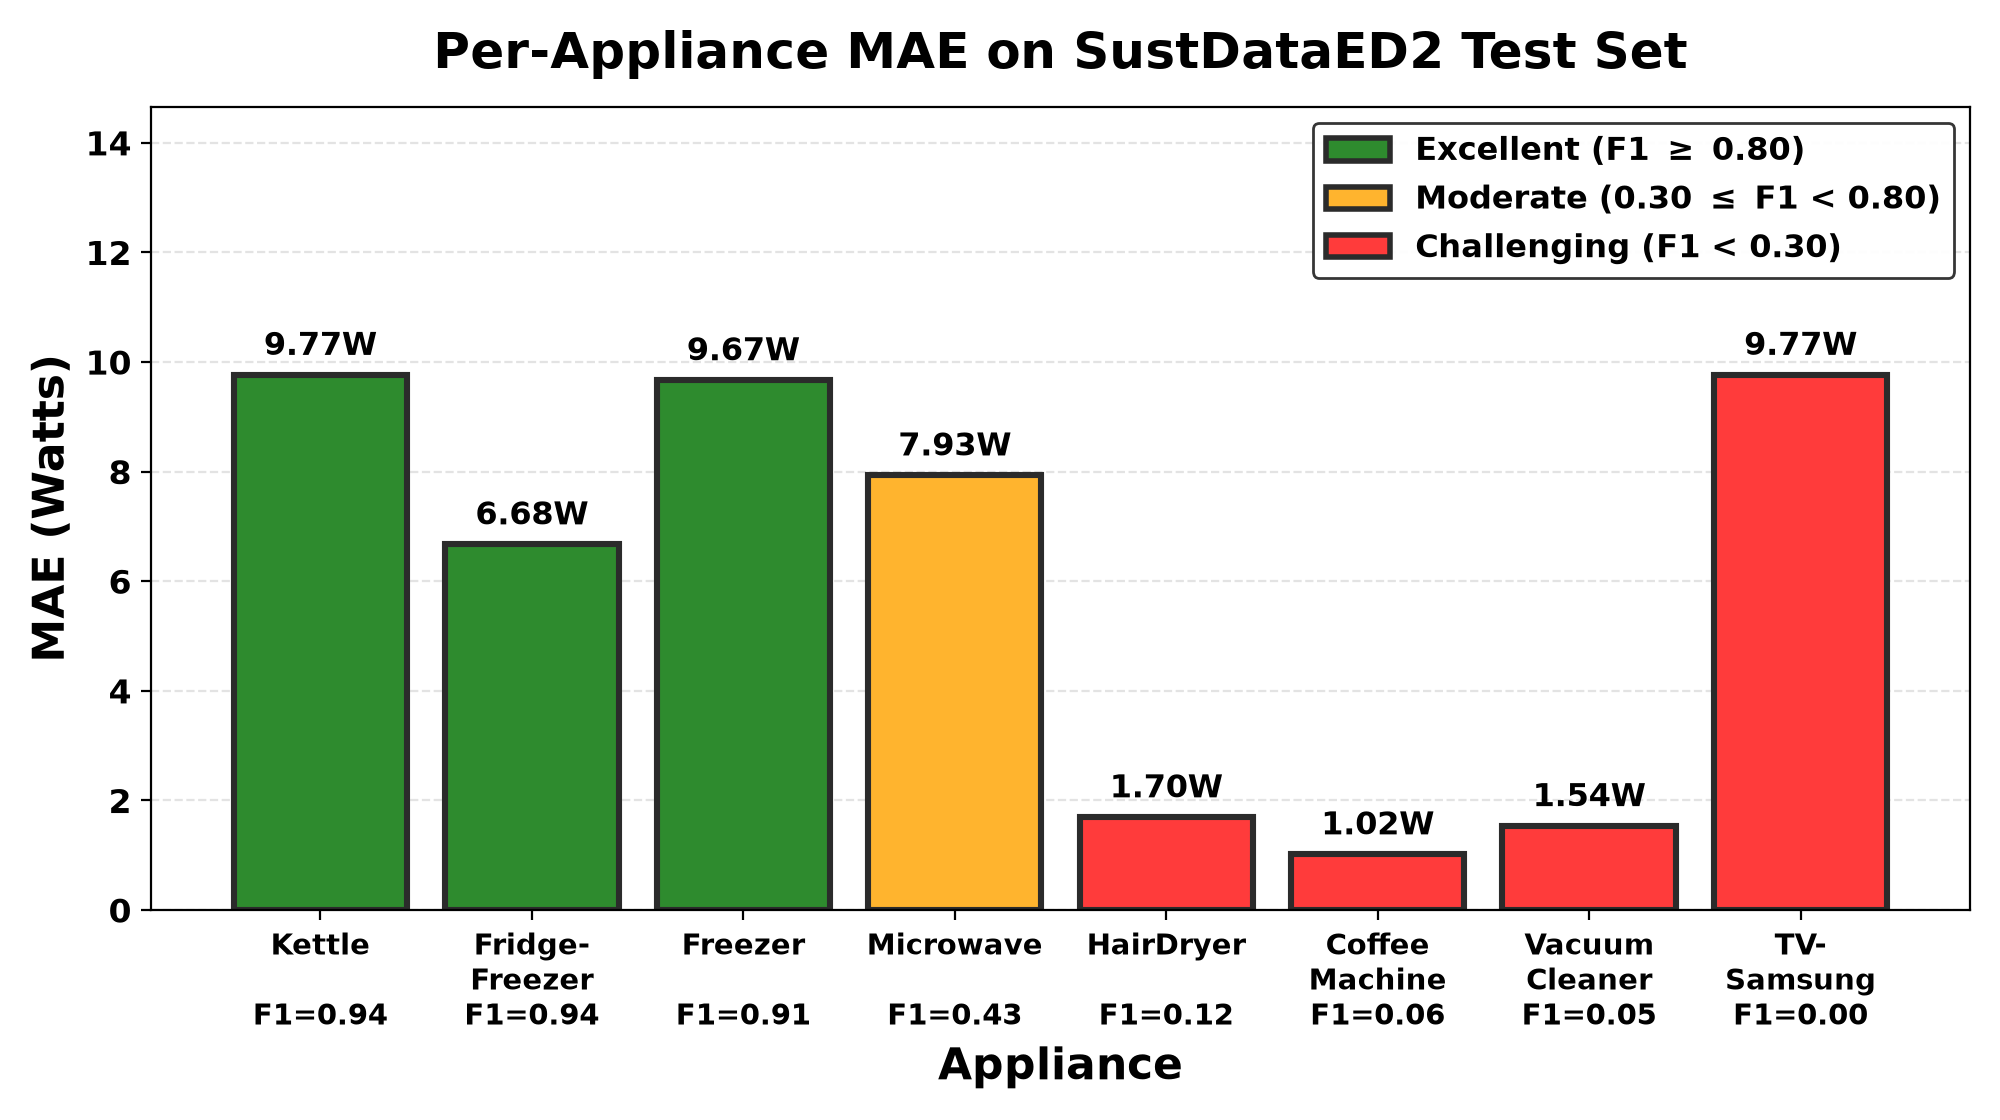
\includegraphics[width=0.60\textwidth]{figures/SustDataED2_per_appliance_mae.png}
\caption{Per-appliance MAE of the deployed model on the SustDataED2 test set, for the appliances that are ON at least once in the test split (bars colored by the F1 at 15~W, which is also printed under each appliance). Fridge-Freezer, Freezer and Kettle are detected reliably; low-power and rarely active appliances remain challenging.}
\label{fig:SustDataED2_results}
\end{figure}

\begin{table}[H]
\centering
\caption{Binary classification evolution on REFIT through systematic loss function optimization. Weighted BCE addresses class imbalance (+41\% F1), while excluding the kettle and the tumble dryer, for which no usable classifier could be trained, prevents numerical instability.}
\label{tab:classification_evolution}
\small
\begin{tabular}{@{}lcccccc@{}}
\toprule
Iteration & Loss Function & Appliances & F1 & Prec. & Recall & Key Improvement \\
\midrule
1 & Unweighted BCE & 9 & 0.394 & 0.410 & 0.384 & Baseline \\
2 & Weighted BCE & 9 & 0.557 & -- & 0.744 & +41\% F1, +94\% Recall \\
3 & Weighted BCE & 7 & 0.60-0.65 & 0.50-0.60 & 0.70-0.80 & Balanced metrics \\
\bottomrule
\multicolumn{7}{l}{\footnotesize Iteration 1: Learns prior distribution (always-OFF bias).} \\
\multicolumn{7}{l}{\footnotesize Iteration 2: Weighted BCE with $w_{pos,a} = (1 - r_a) / r_a$ addresses imbalance.} \\
\multicolumn{7}{l}{\footnotesize Iteration 3: Excludes kettle, tumble dryer (precision 0--4\% at 108{,}000 and 73{,}000 false positives; $w_{pos,a} > 100$ unstable).}
\end{tabular}
\end{table}

\begin{figure}[H]
\centering
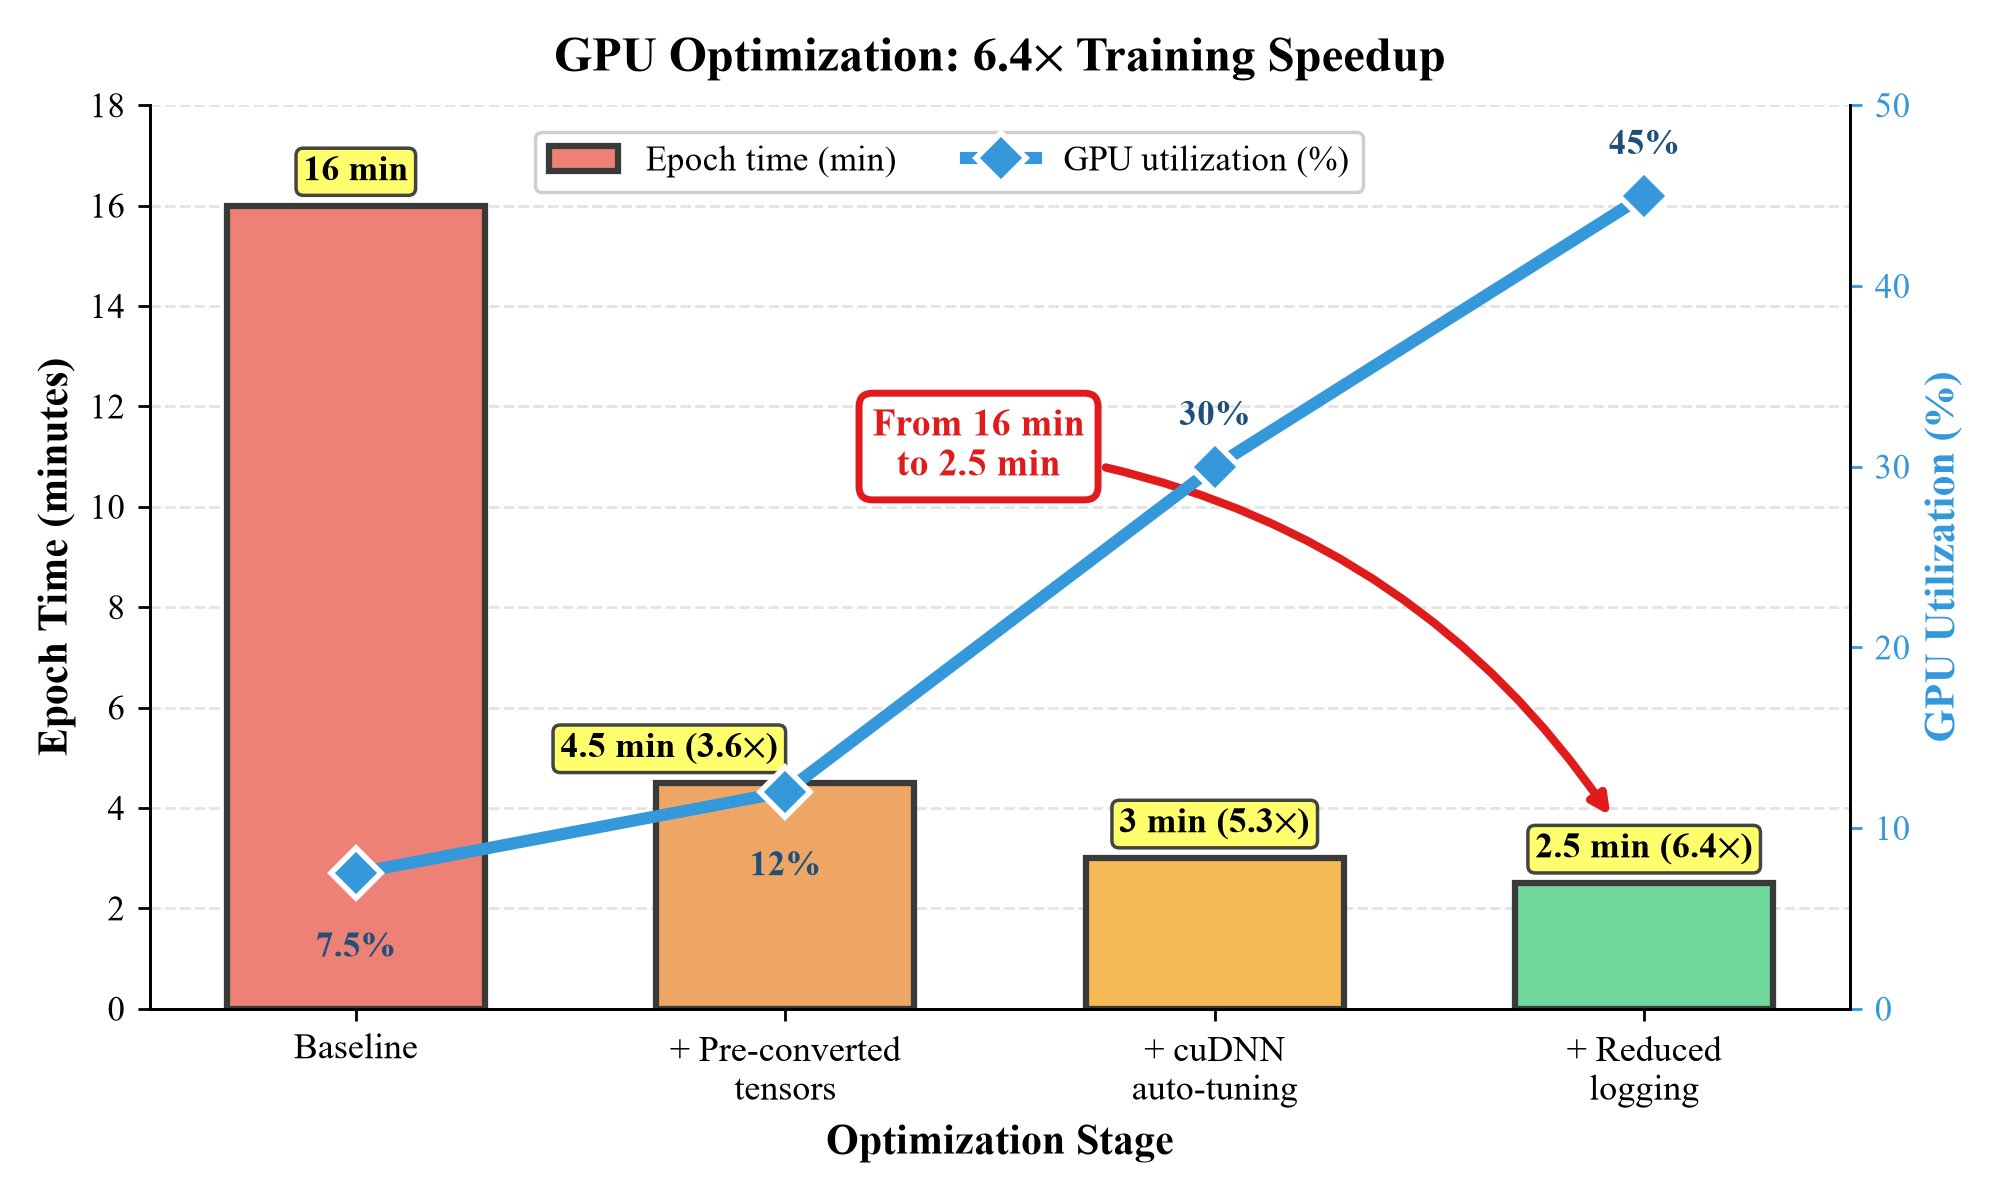
\includegraphics[width=0.60\textwidth]{figures/training_speedup.png}
\caption{Training efficiency improvements through GPU optimization. Sequential optimizations (pre-converted tensors, cuDNN auto-tuning, reduced logging) achieve cumulative $6.4\times$ speedup, reducing epoch time from 16 min to 2.5 min. GPU utilization increases from 5-10\% (memory-bound baseline) to 40-50\% (compute-bound optimized), enabling practical hyperparameter search on 380K-sample datasets.}
\label{fig:training_speedup}
\end{figure}

\begin{table}[H]
\centering
\caption{Post-processing threshold $\tau$ (predictions below $\tau$ are set to OFF; the ground-truth ON threshold stays at 15~W). F1 on the validation and test splits of each dataset; the value selected on the validation split is in bold. The threshold is never tuned on test data.}
\label{tab:threshold_sweep}
\footnotesize
\begin{tabular}{@{}lcccccc@{}}
\toprule
 & \multicolumn{2}{c}{REFIT} & \multicolumn{2}{c}{SustDataED2} & \multicolumn{2}{c}{UK-DALE} \\
\cmidrule(lr){2-3}\cmidrule(lr){4-5}\cmidrule(lr){6-7}
$\tau$ (W) & val F1 & test F1 & val F1 & test F1 & val F1 & test F1 \\
\midrule
0 & 0.432 & 0.163 & 0.138 & 0.143 & 0.181 & 0.247 \\
5 & 0.661 & 0.351 & 0.385 & 0.396 & 0.381 & 0.455 \\
10 & \textbf{0.679} & \textbf{0.409} & 0.765 & 0.772 & 0.455 & 0.509 \\
15 & 0.677 & 0.448 & 0.817 & 0.824 & 0.507 & 0.531 \\
20 & 0.651 & 0.464 & \textbf{0.840} & \textbf{0.845} & 0.560 & 0.534 \\
25 & 0.597 & 0.446 & 0.840 & 0.842 & \textbf{0.562} & \textbf{0.519} \\
30 & 0.515 & 0.379 & 0.827 & 0.828 & 0.523 & 0.486 \\
\bottomrule
\end{tabular}
\end{table}

\begin{table}[H]
\centering
\caption{Per-house results on the REFIT houses that were never used for training (appliances present in each house only). House 18 is the validation house; houses 19--21 form the test split.}
\label{tab:unseen_houses}
\footnotesize
\begin{tabular}{@{}lccccccc@{}}
\toprule
 & & \multicolumn{3}{c}{Deployed checkpoint} & \multicolumn{3}{c}{Retrained EDTCN} \\
\cmidrule(lr){3-5}\cmidrule(lr){6-8}
House & Appl. & MAE (W) & F1 & SAE & MAE (W) & F1 & SAE \\
\midrule
18 (validation) & 8 & 22.4 & 0.68 & 0.38 & 21.8 & 0.68 & 0.46 \\
19 & 5 & 14.9 & 0.55 & 0.40 & 14.2 & 0.58 & 0.42 \\
20 & 9 & 16.8 & 0.53 & 0.21 & 16.0 & 0.58 & 0.30 \\
21 & 6 & 23.4 & 0.52 & 0.25 & 23.5 & 0.47 & 0.27 \\
\bottomrule
\end{tabular}
\end{table}

\begin{table}[H]
\centering
\caption{Leave-one-house-out (LOHO) on REFIT. Each held-out training house is evaluated by a model that never saw it (trained 8 epochs on the other houses) and by the reference model trained on all 16 training houses (25 epochs); only appliances present in the house are scored. The gap includes the difference in training length and is therefore an upper bound of the cost of an unseen house.}
\label{tab:loho}
\footnotesize
\begin{tabular}{@{}lccccccc@{}}
\toprule
 & & \multicolumn{2}{c}{House seen in training} & \multicolumn{2}{c}{Held-out house} & \multicolumn{2}{c}{Gap} \\
\cmidrule(lr){3-4}\cmidrule(lr){5-6}\cmidrule(lr){7-8}
House & Appl. & MAE (W) & F1 & MAE (W) & F1 & $\Delta$MAE & $\Delta$F1 \\
\midrule
2 & 6 & 16.9 & 0.52 & 17.5 & 0.48 & +0.6 & -0.04 \\
5 & 8 & 36.5 & 0.50 & 38.1 & 0.47 & +1.6 & -0.03 \\
9 & 7 & 21.6 & 0.60 & 22.2 & 0.61 & +0.6 & +0.02 \\
13 & 7 & 22.5 & 0.63 & 23.5 & 0.60 & +1.0 & -0.03 \\
16 & 5 & 28.5 & 0.60 & 29.5 & 0.58 & +1.1 & -0.01 \\
\midrule
Mean & & 25.2 & 0.57 & 26.2 & 0.55 & +1.0 & -0.02 \\
\bottomrule
\end{tabular}
\end{table}

\begin{table}[H]
\centering
\caption{Zero-shot transfer and adaptation on the five appliances shared by REFIT and UK-DALE (fridge, washing machine, dishwasher, microwave, kettle; present appliances only). Cells show MAE (W) / F1 on the held-out evaluation block (mean of two seeds). $k$ is the number of days of target data used for adaptation. The last two columns give the change of the MAE on the source dataset (forgetting) after full fine-tuning and after fine-tuning with EWC; the trunk-frozen head adaptation changes it by at most 2.7~W.}
\label{tab:transfer}
\footnotesize
\begin{tabular}{@{}lcccccccc@{}}
\toprule
Method & $k$ & Zero-shot & Scratch & Heads only & Full fine-tune & Full + EWC & Forget. full & Forget. EWC \\
\midrule
\multicolumn{9}{l}{\textit{REFIT$\rightarrow$UK-DALE: UK-DALE house 1}; predict-zero MAE 23.8~W; in-domain model (all target-dataset training data) 18.9 / 0.65} \\
zero-shot & 0 & 24.2 / 0.57 & -- & -- & -- & -- & -- & -- \\
adapted & 1 & -- & 33.7 / 0.12 & 24.0 / 0.58 & 24.0 / 0.61 & 24.0 / 0.59 & +9.8 & +7.9 \\
adapted & 3 & -- & 32.3 / 0.12 & 24.1 / 0.59 & 24.2 / 0.61 & 24.1 / 0.58 & +8.5 & +8.7 \\
adapted & 7 & -- & 31.0 / 0.15 & 24.0 / 0.21 & 22.6 / 0.53 & 22.9 / 0.54 & +8.3 & +8.3 \\
\midrule
\multicolumn{9}{l}{\textit{UK-DALE$\rightarrow$REFIT: house 19}; predict-zero MAE 15.4~W; in-domain model (all target-dataset training data) 15.5 / 0.66} \\
zero-shot & 0 & 16.0 / 0.57 & -- & -- & -- & -- & -- & -- \\
adapted & 1 & -- & 22.8 / 0.45 & 15.6 / 0.59 & 16.9 / 0.58 & 16.2 / 0.61 & +3.0 & +2.1 \\
adapted & 3 & -- & 21.8 / 0.51 & 15.5 / 0.59 & 16.8 / 0.62 & 16.5 / 0.61 & +2.8 & +1.9 \\
adapted & 7 & -- & 20.2 / 0.50 & 15.7 / 0.60 & 15.8 / 0.63 & 15.8 / 0.63 & +3.4 & +3.0 \\
\midrule
\multicolumn{9}{l}{\textit{UK-DALE$\rightarrow$REFIT: house 20}; predict-zero MAE 12.1~W; in-domain model (all target-dataset training data) 12.5 / 0.63} \\
zero-shot & 0 & 15.9 / 0.55 & -- & -- & -- & -- & -- & -- \\
adapted & 1 & -- & 20.0 / 0.31 & 15.5 / 0.56 & 15.7 / 0.49 & 15.3 / 0.54 & +5.3 & +2.3 \\
adapted & 3 & -- & 20.2 / 0.32 & 15.7 / 0.55 & 15.0 / 0.50 & 14.9 / 0.53 & +5.6 & +3.8 \\
adapted & 7 & -- & 16.8 / 0.53 & 14.9 / 0.56 & 13.8 / 0.54 & 13.8 / 0.54 & +4.8 & +4.2 \\
\midrule
\multicolumn{9}{l}{\textit{UK-DALE$\rightarrow$REFIT: house 21}; predict-zero MAE 21.7~W; in-domain model (all target-dataset training data) 23.9 / 0.55} \\
zero-shot & 0 & 32.1 / 0.48 & -- & -- & -- & -- & -- & -- \\
adapted & 1 & -- & 34.7 / 0.05 & 32.2 / 0.48 & 29.4 / 0.47 & 27.7 / 0.49 & +4.1 & +3.6 \\
adapted & 3 & -- & 42.3 / 0.38 & 31.9 / 0.48 & 32.0 / 0.47 & 28.2 / 0.49 & +3.6 & +3.2 \\
adapted & 7 & -- & 42.9 / 0.46 & 29.5 / 0.50 & 30.5 / 0.52 & 26.1 / 0.50 & +6.8 & +7.0 \\
\bottomrule
\end{tabular}
\end{table}

\begin{table}[H]
\centering
\caption{Operator-fusion ablation of the regression models (same weights; REFIT on 3{,}000 evenly spaced test windows, the other datasets on the complete test split). Layers: unfused / BN folded / deployed. INT8 results use ACIQ calibration of all convolutions with the same 500 calibration windows. Latency: one window, one thread, PC, range over the three forms (FP32 / INT8), measured in the same way as in Table~\ref{tab:int8_pc}.}
\label{tab:fusion}
\footnotesize
\begin{tabular}{@{}lcccc@{}}
\toprule
Dataset & Layers & INT8 MAE (W) / F1 (all forms) & INT8 size (MB) unfused / deployed & Latency (ms) \\
\midrule
REFIT & 89 / 76 / 60 & 15.85 / 0.450 & 0.74 / 0.72 & 6.8--7.7 / 6.6--7.0 \\
SustDataED2 & 98 / 85 / 66 & 5.38 / 0.816 & 0.78 / 0.76 & 7.2--7.4 / 6.9--7.1 \\
UK-DALE & 98 / 85 / 66 & 17.30 / 0.528 & 0.78 / 0.76 & 7.6--7.9 / 7.0--7.3 \\
\bottomrule
\end{tabular}
\end{table}

To separate the effect of compiler fusion from that of quantization, each regression network was built in three NCNN forms with identical weights (Table~\ref{tab:fusion}): \textit{unfused} (Convolution, BatchNorm and ReLU as separate layers), \textit{BN folded}, and the \textit{deployed} graph in which the ReLU is also merged into the convolution. The unfused graphs were generated directly from the PyTorch weights because PNNX cannot export them; all three forms reproduce the PyTorch output within $4\times10^{-4}$~W, and \texttt{ncnnoptimize} turns the unfused graph into the same 66-layer deployed graph. Fusion removes one third of the layers (98 to 66 for the 12-appliance models) and 0.9\% of the weight file, and it does not change the accuracy: FP32 and INT8 MAE and F1 are identical to the third decimal in all forms. The PC latency is 6.6--7.9~ms for every form, within the measurement repeatability ($\pm$0.4~ms), so no latency benefit could be shown, and the effect on the F1C200s was not measured. Fusion is thus a lossless graph optimization, and the accuracy changes in this section are caused by quantization alone.

\begin{table}[H]
\centering
\caption{Agreement between the soft-float ARM926EJ-S build and the PC build of the rebuilt INT8 models (50 evenly spaced test windows per model; same NCNN model files). Each cell gives the largest absolute difference / the mean absolute difference of the outputs / the percentage of identical ON/OFF decisions. The ARM build was executed on a PC with an ARM926EJ-S CPU model, not on the F1C200s board.}
\label{tab:arm_build}
\footnotesize
\begin{tabular}{@{}llcc@{}}
\toprule
Dataset & Model (unit) & INT8 all layers (ACIQ) & INT8 mixed precision \\
\midrule
REFIT & Reg. (W) & $1.172$ / $4.0\times10^{-4}$ / 100.000 & $0.246$ / $6.7\times10^{-5}$ / 99.998 \\
SustDataED2 & Reg. (W) & $1.2\times10^{-4}$ / $2.0\times10^{-7}$ / 100.000 & $1.180$ / $3.9\times10^{-4}$ / 100.000 \\
UK-DALE & Reg. (W) & $2.4\times10^{-4}$ / $3.0\times10^{-7}$ / 100.000 & $0.651$ / $8.5\times10^{-5}$ / 100.000 \\
REFIT & Cls. (prob.) & $0.014$ / $9.8\times10^{-6}$ / 100.000 & $0.011$ / $3.1\times10^{-6}$ / 100.000 \\
SustDataED2 & Cls. (prob.) & $0.014$ / $2.5\times10^{-6}$ / 100.000 & $6.1\times10^{-3}$ / $3.2\times10^{-6}$ / 99.999 \\
UK-DALE & Cls. (prob.) & $0.015$ / $1.2\times10^{-5}$ / 99.998 & $0.021$ / $5.2\times10^{-5}$ / 99.997 \\
\bottomrule
\end{tabular}
\end{table}

The NCNN engine was also cross-compiled for the ARM926EJ-S without NEON and with software floating point (\texttt{-mcpu=arm926ej-s -mfloat-abi=soft}, statically linked), so the remaining floating-point operations use soft-float routines (Stage 4). Executed on a PC with an ARM926EJ-S CPU model (not on the F1C200s board) on 50 evenly spaced test windows per model, it reproduces the outputs of the PC build (Table~\ref{tab:arm_build}): the mean absolute difference is below $5\times10^{-4}$ (W or probability), the ON/OFF decisions agree in at least 99.996\% of the output samples, and the largest single difference is 1.2~W (isolated one-step INT8 rounding differences; the outputs are not bit-identical). These runs establish functional agreement only; no timing, power or temperature is derived from them.


\begin{table}[H]
\centering
\caption{Latency budget of the NILM service on the F1C200s (REFIT regression model, 512-step window). ``Derived'' entries follow from the window definition or from operation counts; ``measured'' entries are from the timing runs of Table~\ref{tab:hardware_inference_results}.}
\label{tab:latency}
\footnotesize
\begin{tabular}{@{}p{3.3cm}p{1.9cm}p{4.2cm}@{}}
\toprule
Component & Value & Basis \\
\midrule
Window buffering & 4096~s (68.3 min) & derived: 512 steps $\times$ 8~s \\
Model load & 0.28--0.40~s & measured \\
Pre-processing (scaling of 512 samples) & negligible & derived: 512 scalar operations versus $3.8\times10^{8}$ MACs \\
Inference per window & 101.2--123.5~s & measured, 5 repetitions, spread $<0.03$~s \\
Inference per time step & 0.20--0.24~s & derived: inference time / 512 \\
Post-processing (threshold) & negligible & derived: $512\times A$ comparisons \\
Result payload & about 1~KB per event & design value used in Section~\ref{subsec:scalability} \\
Delay of an interval's result & about 2 min after interval end & derived: inference time (steady state, 15-minute cadence) \\
CPU duty at 15-minute cadence & 11--14\% & derived: inference time / 900~s \\
\bottomrule
\end{tabular}
\end{table}

\subsection*{Harmonic verification and forecasting benchmark}

\begin{table}[H]
\centering
\caption{Verification of the THD estimators on synthetic signals.}
\label{tab:thd_verification}
\begin{tabular}{lcc}
\toprule
Estimator & Max. $|\Delta THD|$ (pp) & Mean $|\Delta THD|$ (pp) \\
\midrule
Harmonic subgroups, IEC 61000-4-7 & \textbf{1.09} & \textbf{0.26} \\
Blackman--Harris FFT, peak picking & 10.92 & 1.06 \\
Notch filter (THD+N) & 3.20 & 0.83 \\
\bottomrule
\end{tabular}
\end{table}

\begin{figure}[H]
    \centering
    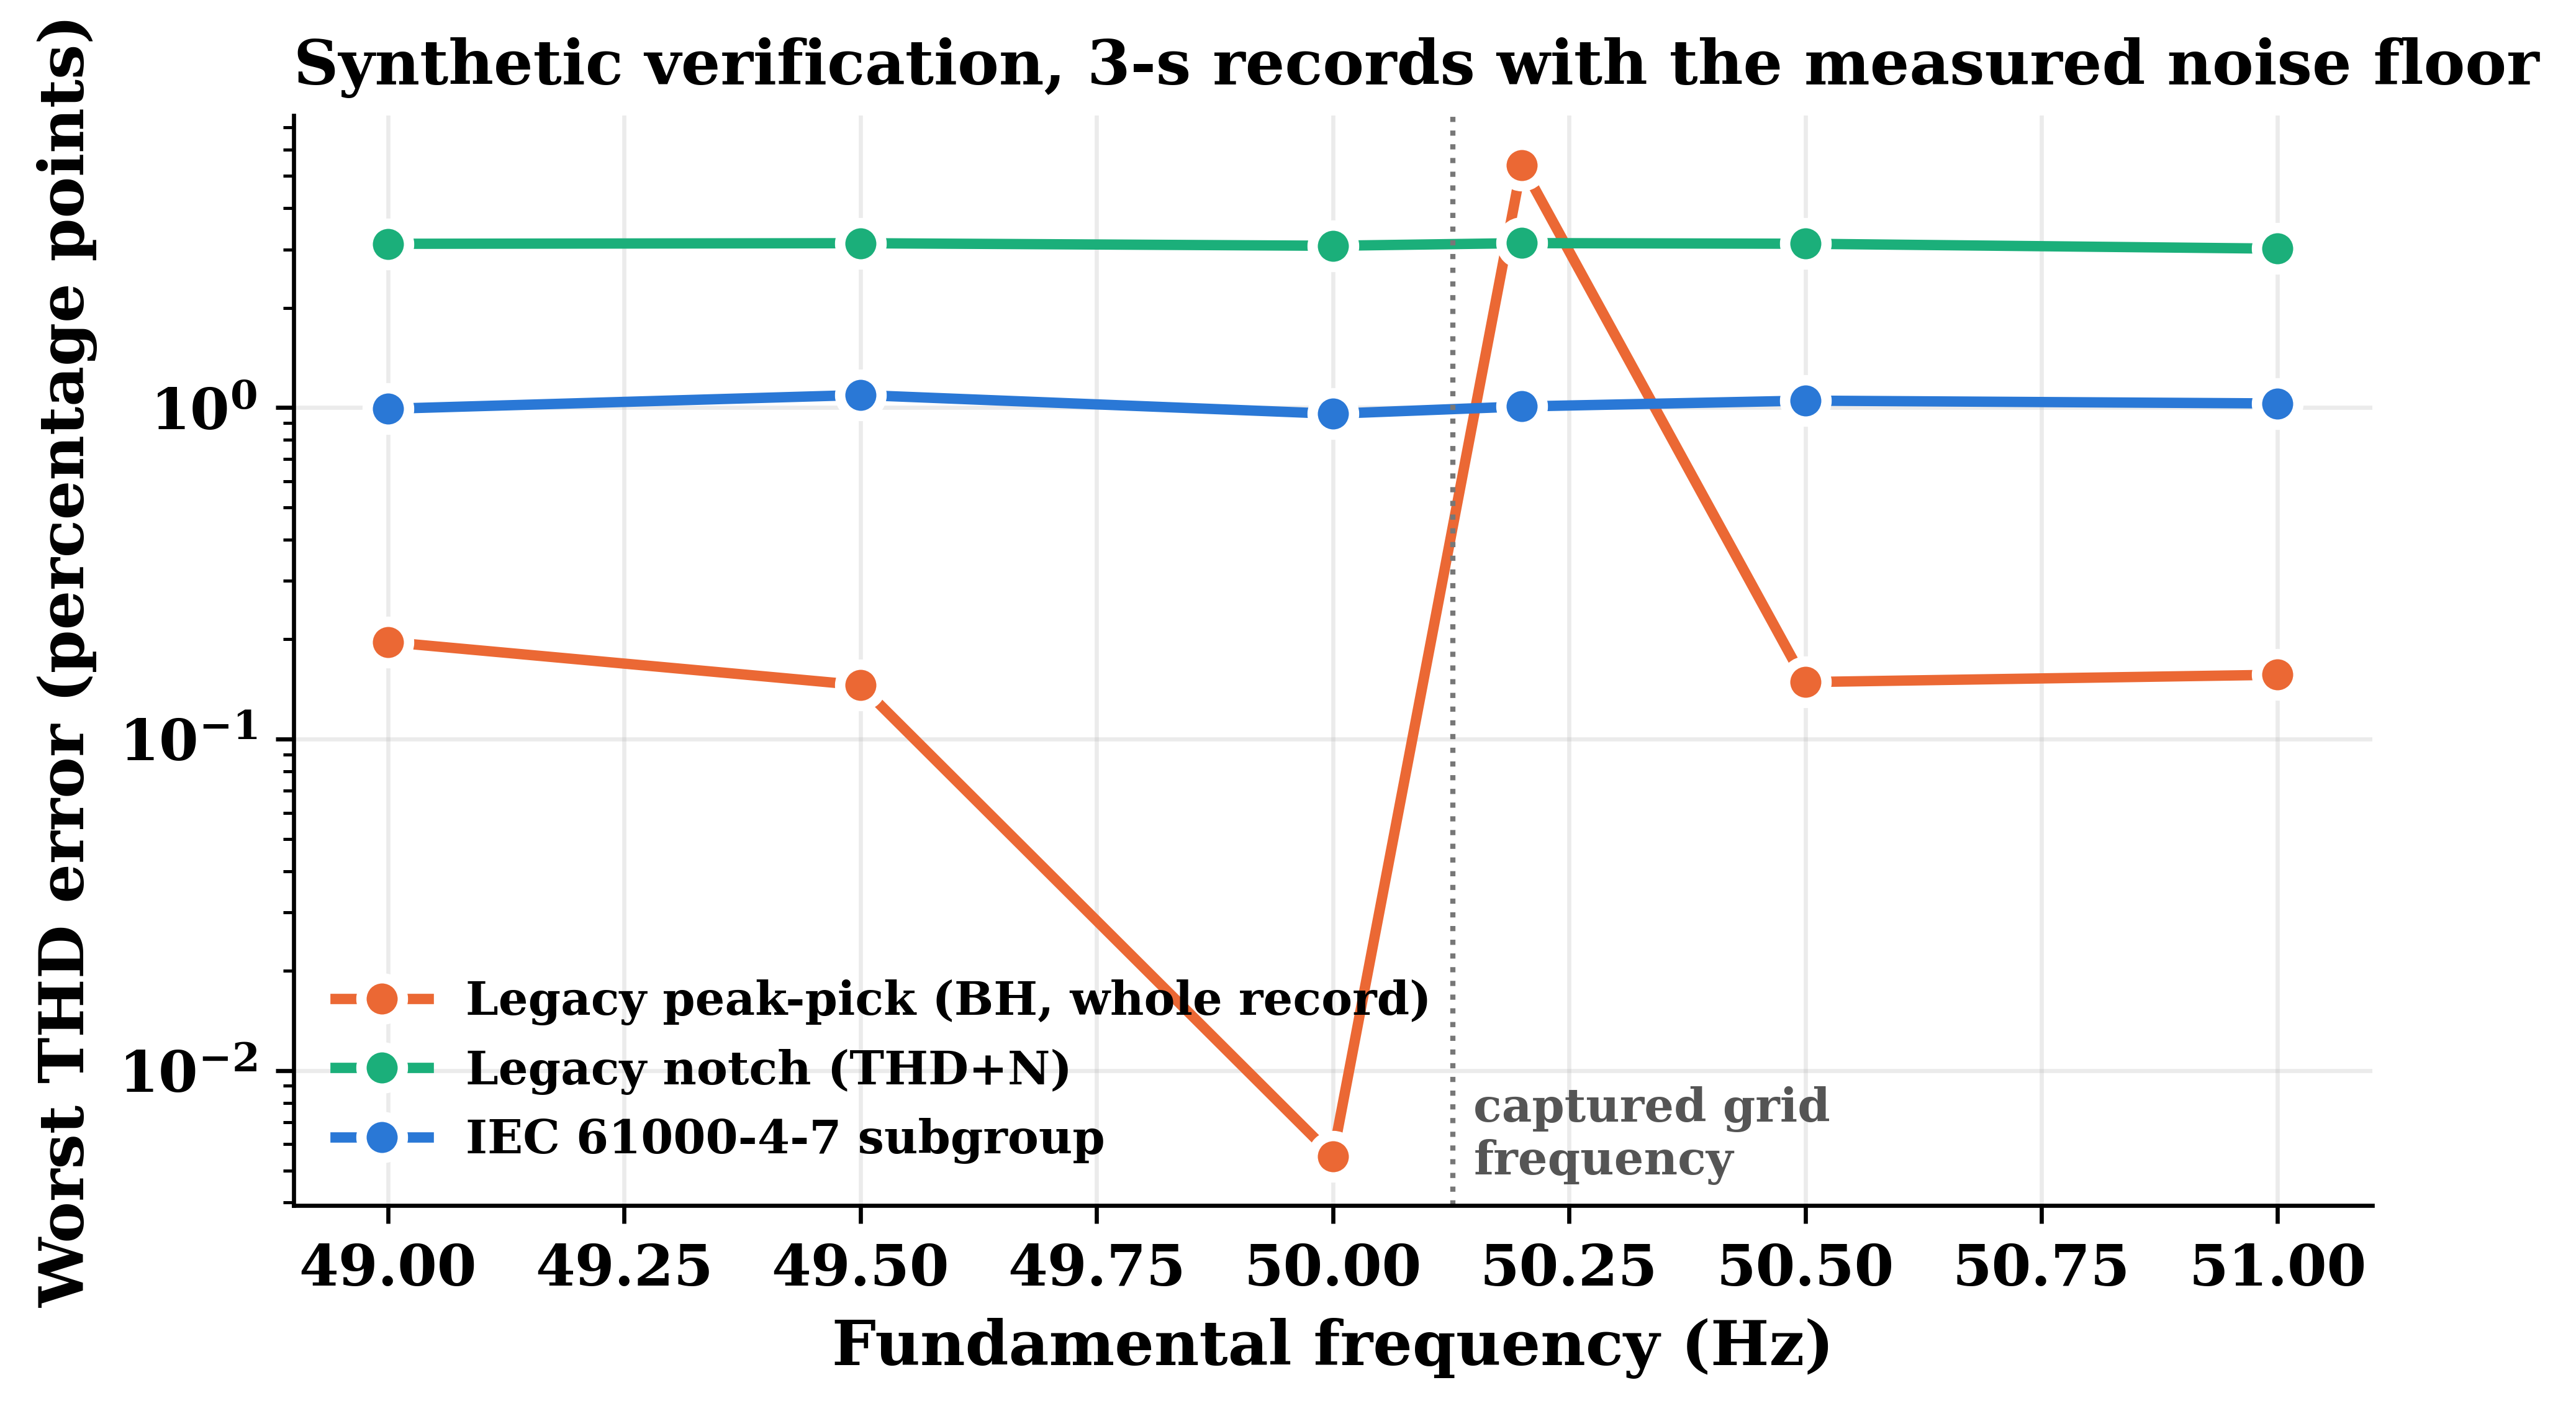
\includegraphics[width=0.75\textwidth]{figures/thd_method_verification.png}
    \caption{Worst-case THD error of the estimators versus fundamental frequency.}
    \label{fig:thd_verification}
\end{figure}

\begin{table}[H]
\centering
\caption{Data splits of the forecasting benchmark.}
\label{tab:forecast_protocol}
\begin{tabular}{lccccc}
\toprule
Split & Period & Intervals & Scored (\%) & Mean (W) & Std (W) \\
\midrule
Train & Apr 2013 -- Mar 2015 & 70{,}080 & 99.3 & 363 & 318 \\
Validation & Apr 2015 -- Mar 2016 & 35{,}136 & 98.0 & 388 & 351 \\
Test & Apr 2016 -- Mar 2017 & 35{,}040 & 98.9 & 396 & 351 \\
\bottomrule
\end{tabular}
\end{table}

\begin{figure}[H]
    \centering
    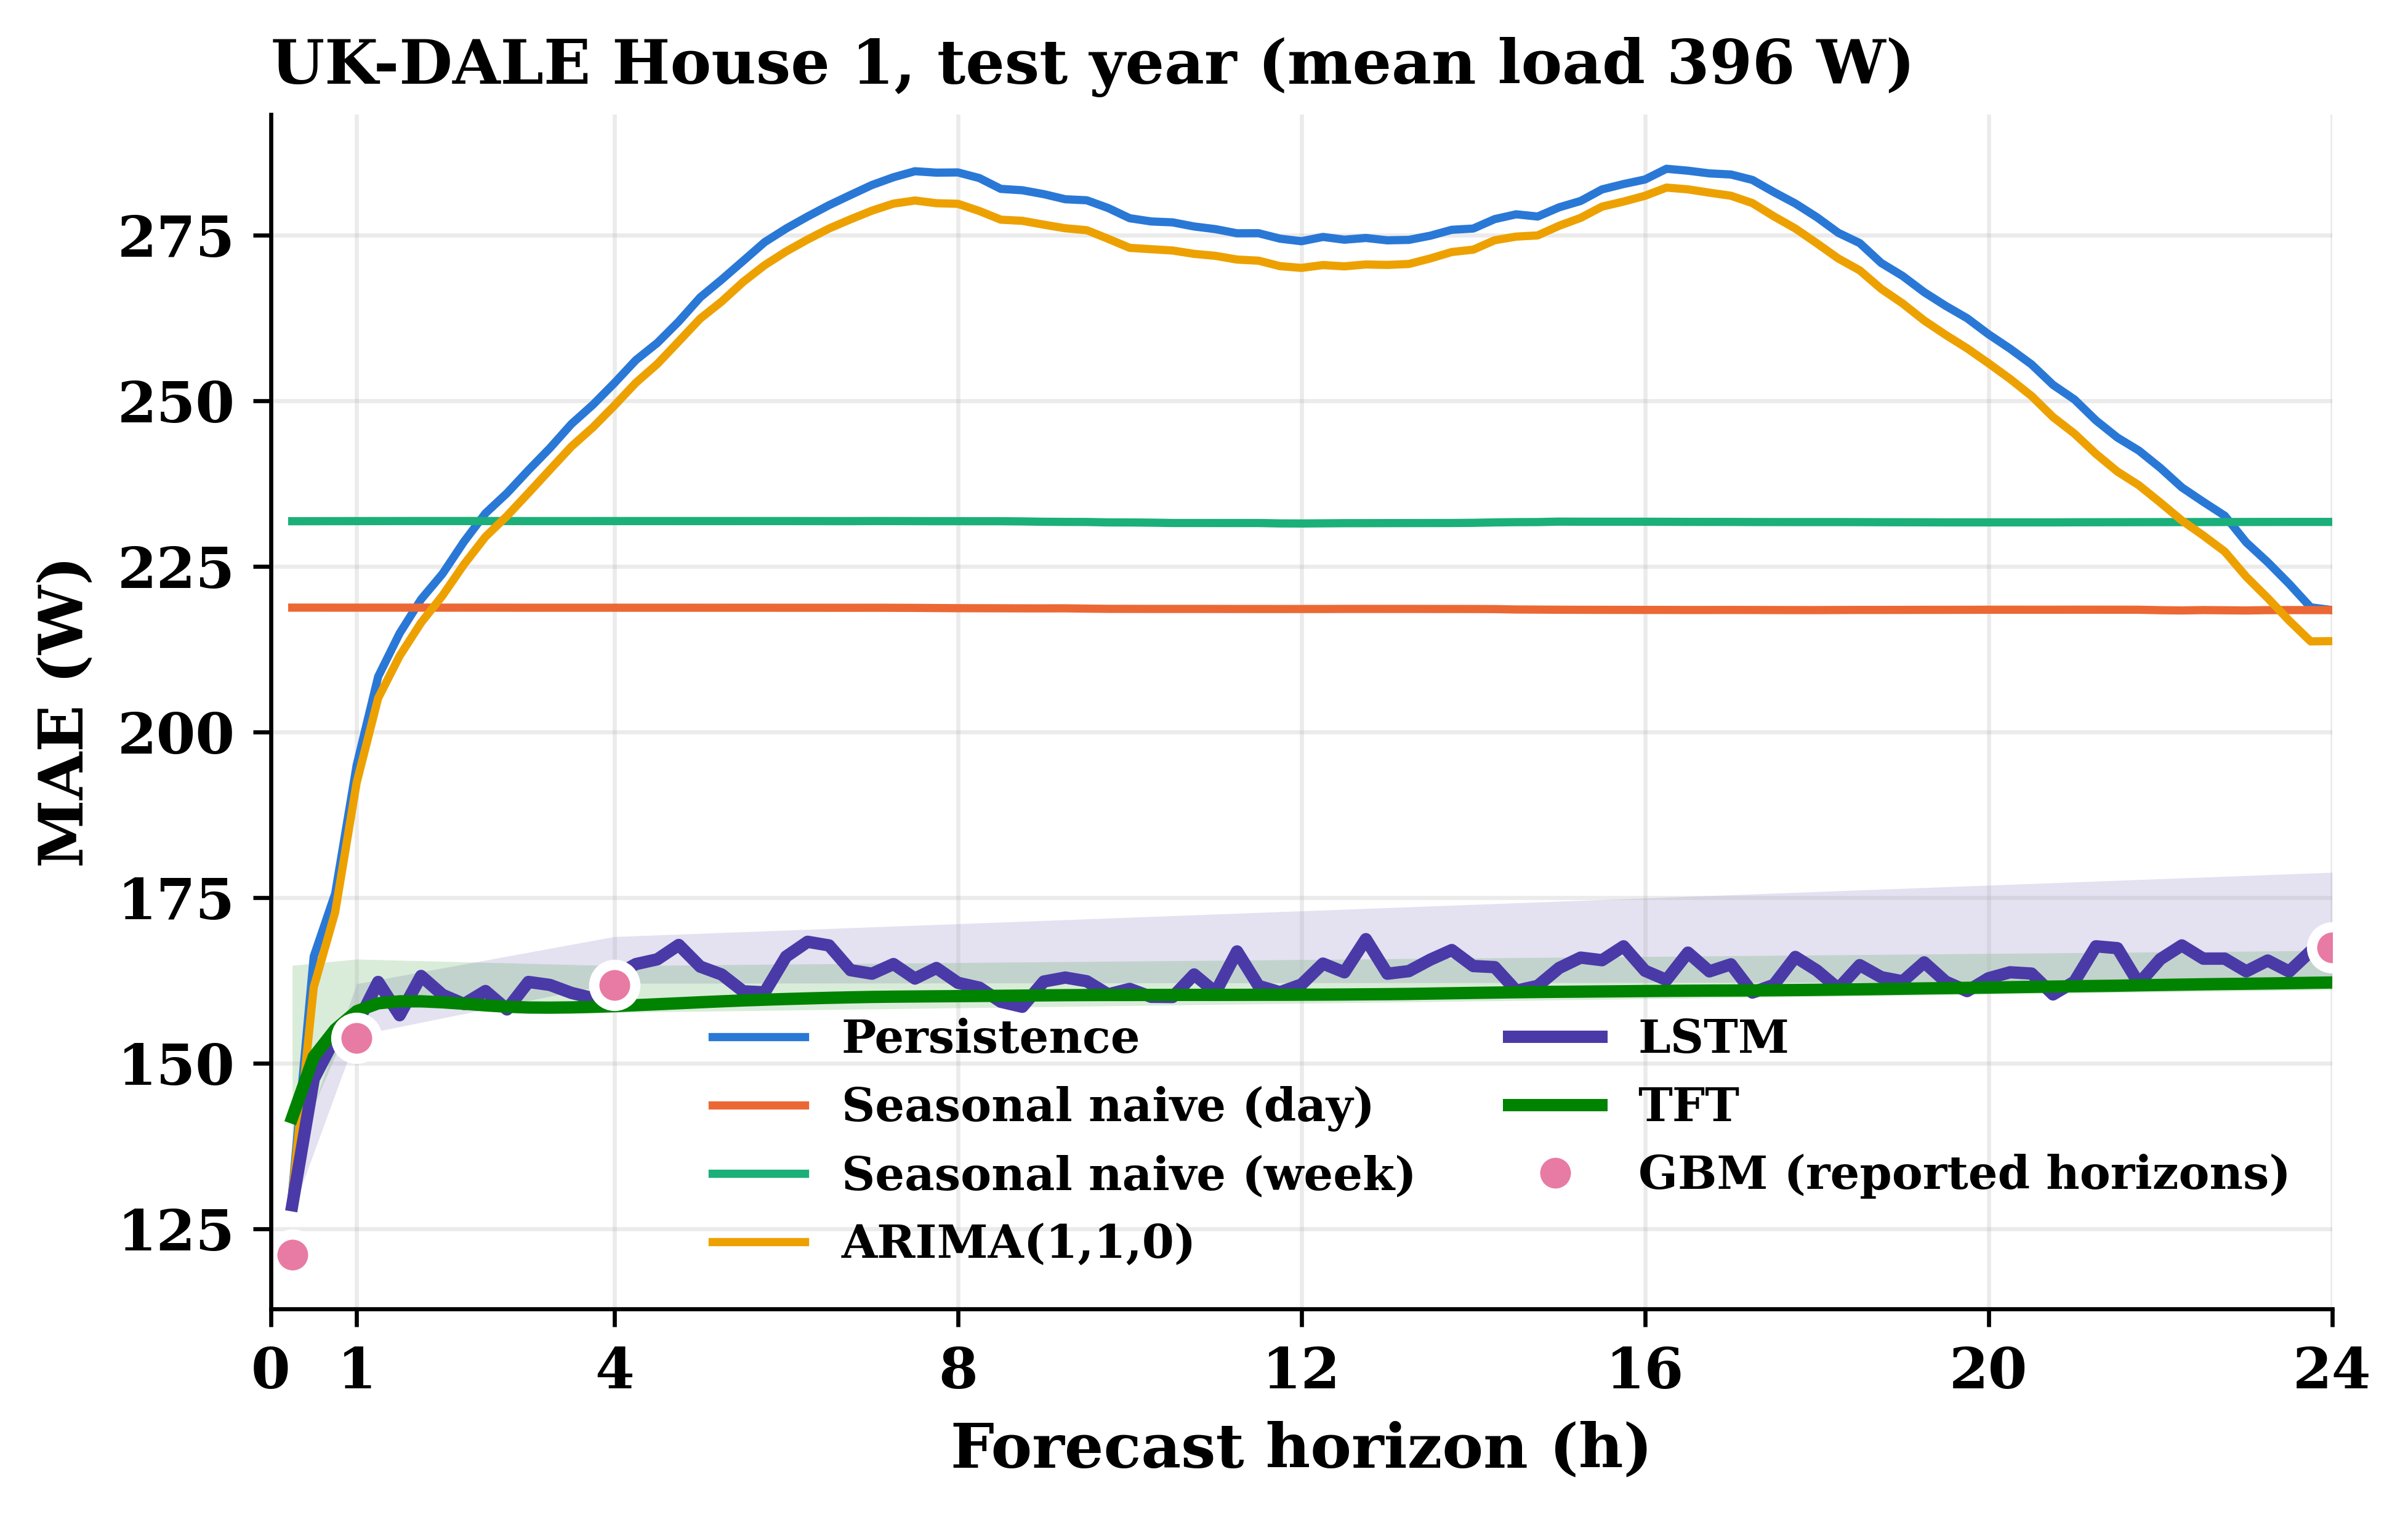
\includegraphics[width=0.85\textwidth]{figures/forecast_mae_vs_horizon.png}
    \caption{Forecast MAE versus horizon on the test year.}
    \label{fig:forecast_horizon}
\end{figure}

\subsection*{Forecast outage analysis and failure modes}

\begin{table}[H]
\centering
\caption{Forecast MAE (W) of the 1-h-ahead forecast during cloud outages, averaged over the outage. The cached forecast covers 24~h at most, so it is not defined for the 3-day outage (--); the hybrid strategy switches to the on-meter ARIMA(1,1,0) forecast when the cached forecast no longer covers the target.}
\label{tab:forecast_outage}
\begin{tabular}{lccc}
\toprule
Outage & Cached cloud forecast & On-meter ARIMA(1,1,0) & Hybrid \\
\midrule
15 min & 155.9 & 192.4 & 155.9 \\
1 h & 159.6 & 192.4 & 159.6 \\
6 h & 162.4 & 192.4 & 162.4 \\
24 h & 164.3 & 192.4 & 164.3 \\
3 days & -- & 192.4 & 183.0 \\
\bottomrule
\end{tabular}
\end{table}

\begin{figure}[H]
    \centering
    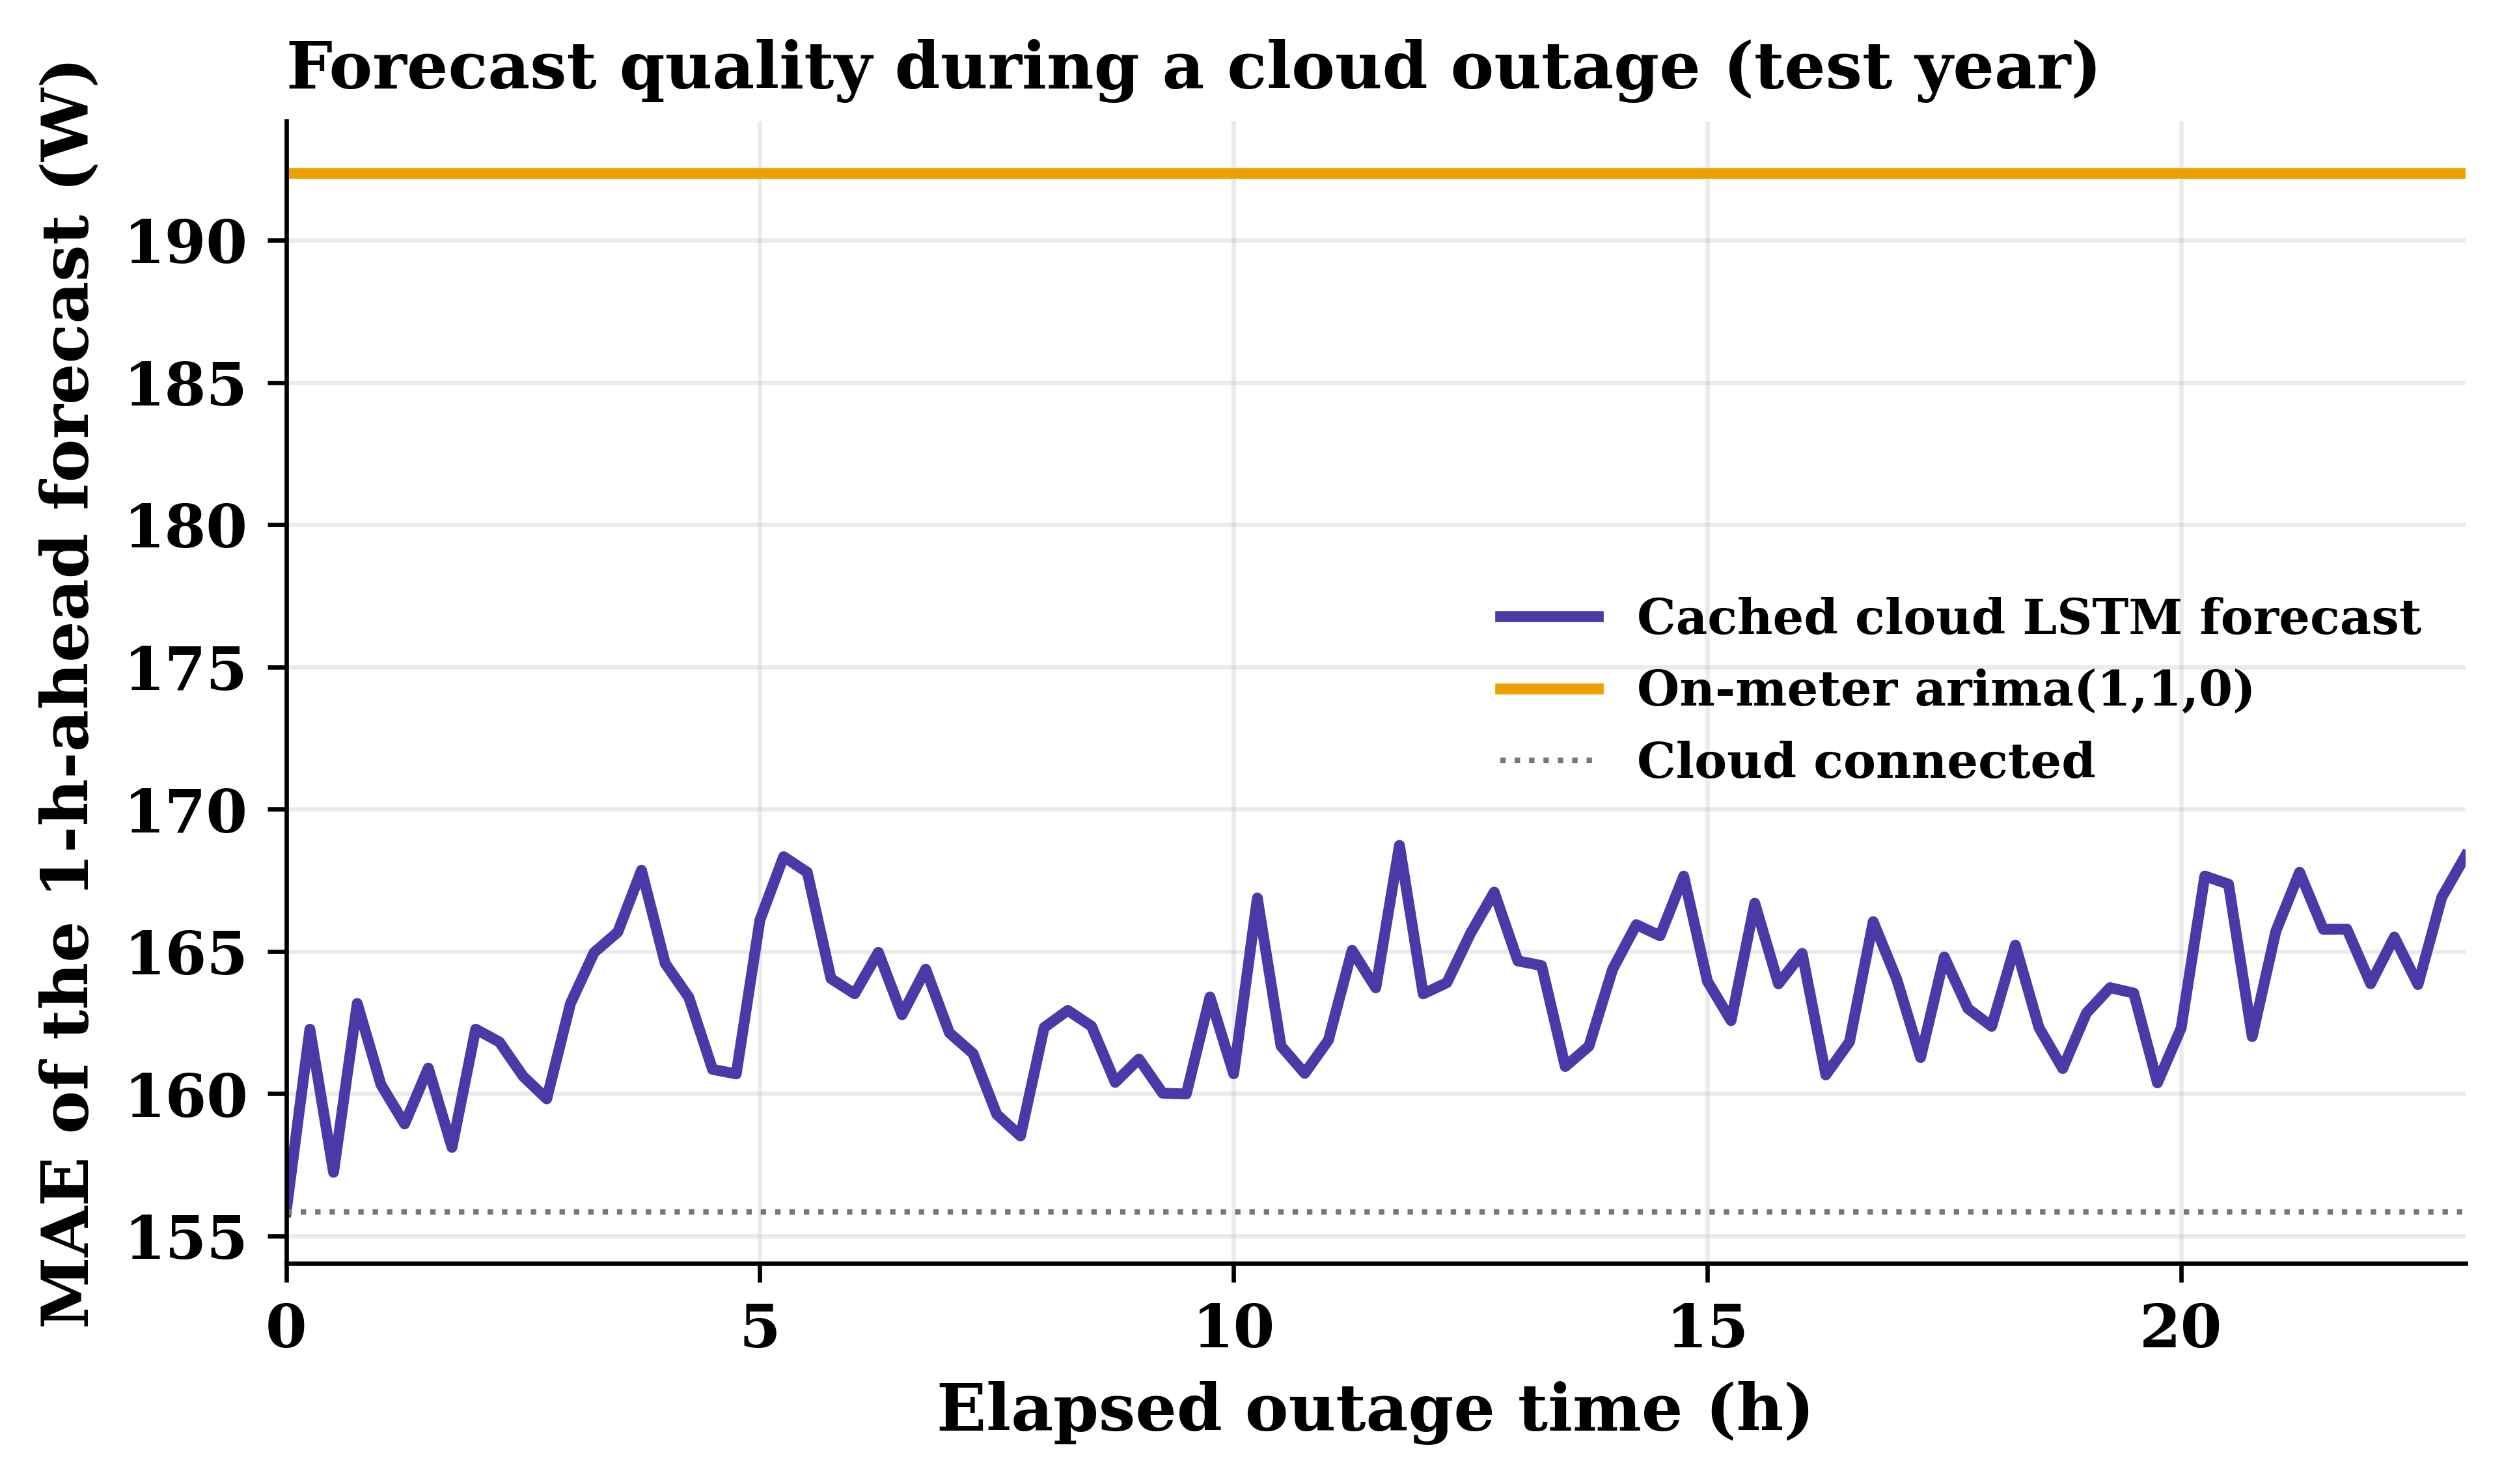
\includegraphics[width=0.75\textwidth]{figures/forecast_cloud_outage.png}
    \caption{Forecast MAE versus elapsed outage time.}
    \label{fig:forecast_outage}
\end{figure}

\begin{table}[H]
\centering
\caption{Failure modes, effect, detection, recovery and status of the prototype.}
\label{tab:failures}
\footnotesize
\begin{tabular}{@{}p{2.6cm}p{3.2cm}p{3.6cm}p{4.2cm}p{1.8cm}@{}}
\toprule
Failure & Effect & Detection & Recovery & Status \\
\midrule
Power outage, unexpected reboot & Metrology and NILM interrupted & At boot, by the file-system journal & Journaling restores file-system integrity; no watchdog or rollback & Partly implemented (OS); watchdog planned \\
NAND / storage corruption & Possible loss of files or model & Kernel storage and MTD layers raise I/O errors (kernel log) & No automatic repair; manual reinstall & Detection implemented; recovery planned \\
SPI failure & Metrology or display data lost & Not instrumented in the prototype & -- & Planned \\
Model or binary corruption & Inference cannot run & Loading or parsing error in user space prevents erroneous execution & Manual reinstall; automated rollback not available & Detection implemented; recovery planned \\
Connectivity loss, cloud interruption & Results cannot be delivered; forecasts unavailable & Connection state & Results buffered in local memory within a capacity and time window; older detail aggregated; duplicates checked after reconnection & Implemented \\
Backend outage & As above & As above & Only local buffering; no further recovery framework & Planned \\
Incorrect NILM prediction & Wrong appliance information shown to the user & Like/dislike feedback in the application, logged for future model improvement (no confidence estimate) & None automatic & Feedback implemented; confidence flag planned \\
\bottomrule
\end{tabular}
\end{table}




\subsection*{Privacy and security details}

\textit{Privacy.} Raw high-frequency voltage and current are processed on the meter and are not uploaded during normal NILM operation; the head-end system receives appliance classifications, estimated appliance power or energy, event timestamps, aggregated consumption and the identifier needed to associate them with an account, and the forecasting service uses only aggregated 15-min values. This reduces the exposure of raw measurements but does not prevent inference of occupancy and routines from appliance-level events, so NGSM is a privacy-risk-reduction architecture, not a guarantee of anonymity. Table~\ref{tab:privacy_threats} summarizes the main threats. Federated learning limits the centralization of training data but adds communication, synchronization and local-training costs on a 64~MB meter without FPU, and its updates can leak information; homomorphic encryption and secure aggregation protect specific computations at the cost of computation, message size and key management that would have to be measured on the target hardware. None of these approaches prevents inference from legitimately shared outputs; combining local inference with secure aggregation for future multi-meter learning is a possible direction.

\begin{table}[H]
\centering
\caption{Main privacy threats, mitigation and residual risk.}
\label{tab:privacy_threats}
\footnotesize
\begin{tabular}{@{}p{2.3cm}p{3.1cm}p{3.5cm}@{}}
\toprule
Threat & Mitigation & Residual risk \\
\midrule
Cloud database compromise & Raw waveforms stay on the meter; data limited to what the service needs; access control & Appliance-level records still reveal routines \\
Unauthorized account access & JWT authentication, protected API routes, authorization checks & Stolen credentials expose a user's data \\
Network interception & TLS and authenticated endpoints & Compromised endpoints or wrong certificate validation \\
Inference from NILM outputs & Limit access; coarser timestamps or aggregation where possible & Sparse events can still reveal behavior \\
Compromised meter, insider misuse, long retention & Firmware hardening, authenticated updates, tamper monitoring, least-privilege roles, retention schedule & Physical access, embedded vulnerabilities, authorized misuse \\
\bottomrule
\end{tabular}
\end{table}

\textit{Web and mobile security.} Authorization is enforced on the server: every backend endpoint validates the JWT signature and expiry, checks that a user can read only the data of their own meter and billing account, and restricts administrative routes by role. Access tokens are short-lived; refresh tokens are rotated and can be revoked. In the browser the tokens are held in secure, HTTP-only cookies, and the mobile application uses the secure storage of the platform. All traffic between the clients, the meters and the server is protected with TLS. Card details are processed by Stripe and are not stored on the servers of the platform, which reduces the PCI-DSS scope of the platform; this does not by itself establish independent PCI-DSS compliance or certification, and none is claimed.

\textbf{Cybersecurity Limitations and Future Work.} The prototype uses JWT-based authentication for protected web routes and API-backed consumption data, TLS, and physical enclosure-tampering detection; these measures are not a complete cybersecurity assurance framework, and the embedded Linux platform and cloud-connected architecture remain exposed to unauthorized access, compromised credentials, malicious firmware and network-level attacks. Future work includes penetration testing of the firmware, communication interfaces, backend APIs and applications; cryptographic signature verification of firmware updates; device identities with mutual authentication; secure boot and a verified update chain, subject to bootloader support on the F1C200s; and centralized security-event monitoring and alerting. These measures will be evaluated through security testing and resource-overhead measurements before being claimed as implemented.

\subsection*{Verification of the harmonic estimator on synthetic signals}

The estimator was verified on synthetic voltage and current signals with known harmonic content, generated at the 44~kHz rate of the prototype capture described below (3-s records). Seven harmonic profiles were used, from a low-distortion profile (6.2\% THD) to an SMPS-like profile (110\% THD), including profiles matching the measured current and voltage spectra. The signals had random harmonic phases, fundamental frequencies from 49 to 51~Hz, a frequency drift of 0.5~Hz within the record, a 1\% interharmonic at 175~Hz, and band-limited noise at the level measured on the prototype. The results are reported in the main text (Table~\ref{tab:thd_verification} and Figure~\ref{fig:thd_verification}).

\subsection*{Cross-checks of the prototype measurement}

In addition to the synthetic verification, the prototype measurement was cross-checked in three ways that do not depend on the FFT implementation (Table~\ref{tab:thd_consistency}). First, an independent estimator that fits sine and cosine terms at $h f_1$ ($h = 1, \dots, 40$) directly to the raw samples of each window by least squares, in the manner of IEEE Std 1057 \cite{ieee1057}, agrees with the subgroup result within 0.003~pp for $THD_V$ and 0.37~pp for $THD_I$. Second, the active power computed in the time domain (46.71~W) equals the sum of the per-harmonic active powers $\sum_h V_h I_h \cos\varphi_h$ within 0.02\%, which checks the amplitudes and the relative phases of both channels. Third, the in-band current noise (13.0~mA) is 25 times larger than the quantization noise of the converter (0.53~mA), so it originates in the analog front end rather than in the digitization. At this light load the noise amounts to 5.8\% of the fundamental current and, together with the fluctuating operation of the load, causes the window-to-window variation of $THD_I$ (standard deviation 1.6~pp over 200-ms windows).

\begin{table}[H]
\centering
\caption{Consistency checks of the prototype measurement.}
\label{tab:thd_consistency}
\begin{tabular}{lc}
\toprule
Check & Value \\
\midrule
$THD_V$: subgroup DFT vs.\ least-squares fit & 0.003~pp \\
$THD_I$: subgroup DFT vs.\ least-squares fit & 0.37~pp \\
Largest difference in $I_h$ ($h \le 15$) & 1.01~pp of $I_1$ \\
Active power, time domain & 46.71~W \\
Active power, sum over harmonics & 46.70~W \\
Power closure error & $-0.02$\% \\
Harmonic active power $P - P_1$ & $-0.005$~W \\
In-band current noise & 13.0~mA \\
Quantization noise (step$/\sqrt{12}$) & 0.53~mA \\
\bottomrule
\end{tabular}
\end{table}

\subsection*{Uncertainty budget of the THD measurement}

The uncertainty of the reported THD values was evaluated following the Guide to the Expression of Uncertainty in Measurement (GUM) \cite{jcgm100} with Monte Carlo propagation \cite{jcgm101} (Table~\ref{tab:thd_uncertainty}). The budget combines the window-to-window repeatability (Type A); the frequency response of the current transformer, bounded by 1\% up to 1.5~kHz and 3\% at 2.5~kHz according to an independent test of split-core metering current transformers \cite{oem_ct_report}; the frequency response of the voltage sensor, whose behaviour above 60~Hz is not specified in its datasheet and for which a bound of $\pm$2\% up to 2~kHz is assumed; the measured noise floor; and the estimator error obtained from the synthetic verification for the measured spectra. The result is $THD_V = 2.15 \pm 0.03\%$ and $THD_I = 35.02 \pm 0.84\%$ (expanded uncertainty, $k = 2$). Repeatability dominates the current uncertainty, which reflects the load and the light-load noise rather than the estimator.

\begin{table}[H]
\centering
\caption{Uncertainty budget of the THD measurement. The combined values come from the Monte Carlo propagation, not from the quadrature sum of the rows.}
\label{tab:thd_uncertainty}
\begin{tabular}{lcc}
\toprule
Source & $u(THD_V)$ (pp) & $u(THD_I)$ (pp) \\
\midrule
Repeatability (Type A) & 0.002 & 0.341 \\
Voltage sensor response & 0.012 & -- \\
Current transformer response & -- & 0.166 \\
Noise floor & 0.002 & 0.074 \\
Estimator (synthetic verification) & 0.005 & 0.183 \\
Combined & 0.013 & 0.419 \\
\midrule
Result ($k = 2$) & $2.15 \pm 0.03\%$ & $35.02 \pm 0.84\%$ \\
\bottomrule
\end{tabular}
\end{table}

\subsection*{Forecasting models: configuration}

Four reference forecasts that require little or no training serve as baselines: persistence (the last observed value), seasonal naive forecasts that repeat the value of the same interval one day or one week earlier, and the Auto-Regressive Integrated Moving Average model ARIMA(1,1,0) of the original NGSM design, fitted on the training years. Three learned models are compared with them. The first consists of gradient-boosted regression trees (GBM) with histogram-based boosting \cite{Ke2017lightgbm, Pedregosa2011sklearn}, with one model per reported horizon; its features are the most recent values and the 1-h and 24-h means, the values of the target interval one, two and seven days earlier, and calendar features of the target interval (time of day, day of week, weekend flag and month). The second is the stacked Long Short-Term Memory (LSTM) network of the NGSM design, with hidden sizes 64, 32 and 16, batch normalization and dropout 0.2, which takes the last two days (192 intervals) of power and calendar features as input and predicts all 96 horizons at once; its output layer additionally receives the values of the same 96 intervals one day and one week earlier. The third is a Temporal Fusion Transformer (TFT) \cite{Lim2021tft}, implemented with Darts \cite{Herzen2022darts}, with hidden size 64, one LSTM layer, four attention heads and dropout 0.3, which uses the same two-day input and 96-step output as the LSTM and receives the calendar features as known future inputs. The LSTM and TFT are trained with the mean squared error on min--max scaled data, excluding unscored intervals from the loss, with early stopping on the validation year and restoration of the best epoch. Each learned model is trained with five random seeds. Table~\ref{tab:forecast_repro} lists the complete configuration.

\begin{table}[H]
\centering
\caption{Configuration of the forecasting models.}
\label{tab:forecast_repro}
\small
\begin{tabular}{l p{13.2cm}}
\toprule
Model & Configuration \\
\midrule
All & 15-min mean active power; train / validation / test: Apr 2013--Mar 2015 / Apr 2015--Mar 2016 / Apr 2016--Mar 2017; min--max scaling fitted on the training years; unscored intervals excluded from losses and metrics; forecasts of 1--96 intervals from every origin. \\
Baselines & Persistence; seasonal naive with periods of 1 and 7 days; ARIMA(1,1,0) fitted on the training years ($\phi = -0.26$) with closed-form $h$-step forecasts. \\
GBM & Histogram gradient boosting (scikit-learn), one model for each of the horizons 1, 4, 16 and 96 intervals; learning rate 0.05, 63 leaves, L2 regularization 1.0, at most 600 iterations with early stopping (10\% internal validation, 30 rounds); 5 seeds. \\
LSTM & LSTM layers 64--32--16 with batch normalization and dropout 0.2; dense output of 96 values that also receives the same intervals 1 and 7 days earlier; input of 192 intervals $\times$ 5 features (scaled power; time of day and day of week as sine/cosine); NAdam, learning rate $10^{-3}$ halved on validation plateau (patience 2), batch 256, at most 60 epochs, early stopping patience 6, gradient clipping 1.0; 5 seeds. \\
TFT & Darts TFTModel: hidden size 64, 1 LSTM layer, 4 attention heads, dropout 0.3; input 192, output 96 intervals; known future covariates: time of day, day of week and month (sine/cosine); mean squared error loss; Adam, learning rate $10^{-3}$, batch 256, at most 40 epochs, early stopping patience 5, best epoch restored; 5 seeds. \\
\bottomrule
\end{tabular}
\end{table}

\subsection*{Forecasting models: computational cost}

\begin{table}[H]
\centering
\caption{Computational cost of the forecasting models.}
\label{tab:forecast_compute}
\small
\begin{tabular}{lccccc}
\toprule
Model & Parameters & Size & Latency & Meters per core & Training per seed \\
\midrule
GBM & -- & -- & 5.4~ms per horizon & $\approx$83{,}000\textsuperscript{a} & $\approx$5~s per horizon \\
LSTM & 54{,}208 & 212~kB & 2.1~ms (96 horizons) & 432{,}758 & 1.4~min \\
TFT & 230{,}061 & 899~kB & 73.6~ms (96 horizons) & 12{,}229 & $\approx$45~min \\
\bottomrule
\multicolumn{6}{l}{\footnotesize \textsuperscript{a} 15-min and 1-h models (two predictions per meter and interval).} \\
\end{tabular}
\end{table}


\subsection*{Reproducibility Details of the NILM Experiments}
Table~\ref{tab:repro} lists the software versions, the window counts of the chronological splits (one window is 512 samples at 8~s) and the checksums of the six deployed checkpoints, so that the reported results can be traced to the exact files used. Training seeds (2026--2030), the optimizer settings, the 500-window calibration sets, the 15~W state threshold and the bootstrap settings are given in the main text. The hardware used for training was an NVIDIA RTX 3050 6~GB laptop GPU, and the INT8 evaluation on the PC used the NCNN CPU back end with one thread per process.

\begin{table}[H]
\centering
\caption{Software versions, split sizes and checksums of the deployed checkpoints.}
\label{tab:repro}
\footnotesize
\begin{tabular}{@{}p{2.3cm}p{5.7cm}@{}}
\toprule
\multicolumn{2}{l}{\textit{Software}} \\
Environment & Python 3.12.0, PyTorch 2.6.0 (CUDA 12.4), NumPy 1.26.4 \\
Deployment & PNNX 20260526, NCNN 1.0 (build 20260526) \\
\midrule
\multicolumn{2}{l}{\textit{Windows per split (train / validation / test)}} \\
REFIT & 380{,}224 / 18{,}689 / 59{,}927 \\
SustDataED2 & 1{,}416 / 303 / 304 \\
UK-DALE & 11{,}610 / 2{,}488 / 2{,}488 \\
\midrule
\multicolumn{2}{l}{\textit{SHA-256 of the checkpoint files (first 16 hexadecimal digits)}} \\
REFIT, regression & f3e16762ce763163 \\
SustDataED2, regression & 6739d309cffd5585 \\
UK-DALE, regression & 6c743e9c7c331a78 \\
REFIT, classification & b5408c030b2b4508 \\
SustDataED2, classification & 1ac6a0a9d5136d90 \\
UK-DALE, classification & 4a8d8dfc9bf5f326 \\
\bottomrule
\end{tabular}
\end{table}
